\documentclass[12pt]{scrreprt} % Set font size to 12pt

\usepackage{changepage} % Add the changepage package for the addmargin environment
\usepackage{blindtext} % Generate lorem ipsums
\usepackage{helvet} % Arial font (Arial is proprietary, so we use Helvetica instead)
\renewcommand{\familydefault}{\sfdefault}
\usepackage[margin=2.5cm]{geometry} % Set margins to 2.5cm on all sides
\usepackage{graphicx} % Add the graphicx package for including images
\usepackage{atbegshi} % Package for placing elements at absolute positions
\usepackage[allcolors=blue]{hyperref} % Add the hyperref package for hyperlinking
\usepackage{xcolor} % Add the xcolor package for color support
\usepackage{tabularx} % Add the tabularx package for advanced tables


\makeatletter
\def\@cite#1#2{$^{\mbox{\scriptsize [#1\if@tempswa , #2\fi]}}$}
\makeatother

% CONSIGNES POUR LA REDACTION DU RAPPORT DE PROJET

% CRITERES D'EVALUATION :
% Critères liés à votre travail et vos compétences :
% - Le respect des objectifs fixés
% - Les compétences techniques et scientifiques
% - L'aptitude à rechercher de l'information
% - L'implication et l'esprit d'initiative
%
% Critères liés à votre rapport de projet
% - La structuration du document
% - L'orthographe et l'expression écrite
% - Le descriptif de la mission
% - La valeur du contenu scientifique et technique
% - La précision des résumés en français, en anglais et la bibliographie
%
% Critères liés à votre soutenance
% - La qualité de la structuration et de l'expression
% - La qualité du diaporama
% - Le dynamisme et l'interactivité
% - La qualité des réponses, l'esprit critique sur le travail réalisé, qualité de la conclusion et des éventuelles perspectives.

% RAPPORT
% Informations générales
%
% Le rapport doit être rédigé par vos soins, en respectant les normes
% de rédaction indiquées ci-dessous. Il sera évalué sur la forme
% (orthographe, grammaire, ponctuation, langage approprié, etc.) et le fond
% (organisation, méthode, argumentation, etc.).
% Il devra avoir une longueur comprise entre 20 et 25 pages (hors annexes)
% et sera à rendre au format PDF.
% L'ensemble des comptes rendus hebdomadaires d'avancement constituera une rubrique annexe de votre rapport.
% Votre document doit comporter une bibliographie permettant d'identifier et de retrouver les documents cités.
%
% Le rapport est à remettre le 9 avril 2024.
%
% Format attendu du document
% - Police Arial
% - Taille des polices : Texte (12), Sections/Titres (14, gras)
% - Numérotation des sections : numérotation scientifique (1, 1.1, 1.1.1)
% - Numérotation des pages : centrale en bas de page
% - Numérotation des tableaux et des figures
% - Marges : 2,5 cm en haut, en bas, à gauche et à droite
% - Résumé (français) et abstract (anglais) sur la dernière page de couverture
% - La première et la quatrième de couverture doivent respecter scrupuleusement le modèle téléchargeable ci-après
% - La mise en page du corps du rapport est libre.




\begin{document}

% add the 0.jpg image to the top-left of the first page

\begin{titlepage}
    \newgeometry{left=1cm, right=1cm, top=1cm, bottom=1cm}

    \noindent
\includegraphics{0.jpg}
    
\includegraphics{1.jpg}
    \hfill
    
\includegraphics{2.jpg}
    \vspace{1cm}


    École Polytechnique de l'Université de Tours

    64, Avenue Jean

    Portalis 37200

    TOURS, FRANCE

    (33)2-47-36-14-14

    \textcolor{red}{\url{http://www.polytech.univ-tours.fr}}


    \vfill
    \begin{center}

        \Huge
        Parcours des écoles d'ingénieur Polytech
        \vspace{0.3cm}

        \textbf{Année 2023-2024}
        \vspace{0.5cm}


        \textbf{Projet Informatique : Labyrinthe}
    \end{center}
    \vfill

    % footer
    \begin{minipage}[t]{0.5\textwidth}
        \begin{flushleft}
            Étudiants
            \vspace{0.1cm}
            \hrule % horizontal
            \vspace{0.5cm}

            \textbf{Pacôme Renimel--Lamiré}
            \href{mailto:pacome.renimel--lamire@etu.univ-tours.fr}{\textcolor{blue}{pacome.renimel--lamire@etu.univ-tours.fr}}

            \textbf{Esteban Laurent}
            \href{mailto:esteban.laurent@etu.univ-tours.fr}{\textcolor{blue}{esteban.laurent@etu.univ-tours.fr}}
        \end{flushleft}
    \end{minipage}
    \begin{minipage}[t]{0.5\textwidth}
        \begin{flushright}
            Encadrant

            \vspace{0.1cm}
            \hrule % horizontal
            \vspace{0.5cm}

            \textbf{Christophe Lenté}

            \href{mailto:christophe.lente@univ-tours.fr}{\textcolor{blue}{christophe.lente@univ-tours.fr}}

        \end{flushright}
    \end{minipage}
\end{titlepage}
\restoregeometry


\chapter*{Avertissement}
\addcontentsline{toc}{chapter}{Avertissement} % Add the chapter to the table of contents

Ce document a été rédigé par Pacôme Renimel--Lamiré et Esteban Laurent susnommés les auteurs.

L’École Polytechnique de l’Université François Rabelais de Tours est représentée par Christophe Lenté susnommé le tuteur académique.

Par l’utilisation de ce modèle de document, l’ensemble des intervenants du projet acceptent les conditions définies ci-après.


Les auteurs reconnaissent assumer l’entière responsabilité du contenu du document ainsi que toutes suites judiciaires qui pourraient en découler du fait du non-respect des lois ou des droits d’auteur.

Les auteurs attestent que les propos du document sont sincères et assument l’entière responsabilité de la véracité des propos.

Les auteurs attestent ne pas s’approprier le travail d’autrui et que le document ne contient aucun plagiat.

Les auteurs attestent que le document ne contient aucun propos diffamatoire ou condamnable devant la loi.

Les auteurs reconnaissent qu’ils ne peuvent diffuser ce document en partie ou en intégralité sous quelque forme que ce soit sans l’accord préalable du tuteur académique et de l’entreprise.

Les auteurs autorisent l’école polytechnique de l’université François Rabelais de Tours à diffuser tout ou partie de ce document, sous quelque forme que ce soit, y compris après transformation en citant la source.

Cette diffusion devra se faire gracieusement et être accompagnée du présent avertissement.

\newpage
\renewcommand{\contentsname}{Table des matières} % Change the title of the table of contents to "Sommaire"
\tableofcontents


\newpage
\chapter*{Introduction}
\addcontentsline{toc}{chapter}{Introduction} % Add the chapter to the table of contents

% Ajouter un overview du projet
% Expliquer la motivation derrière le choix du sujet du projet : pourquoi est-ce important ? Quels sont les enjeux ?
% Décrire les buts et objectifs du projet
% Mentionner brièvement les algorithmes implémentés

Ce rapport a pour objectifs de décrire les différentes étapes de réalisation d'un programme informatique permettant de générer et résoudre automatiquement des labyrinthes, ainsi que de présenter les résultats obtenus.

L'objectif premier du projet consiste à créer un labyrinthe par une ou plusieurs méthodes différentes et à faire trouver à l'ordinateur un chemin menant vers la sortie. Pour ce faire, nous avons implémenté trois algorithmes différents :
\texttt{depth-first search}, \texttt{recursive backtracking} et \texttt{A*}.

La suite du projet a été laissée relativement libre, nous invitant à faire preuve d'imagination et de créativité pour aller au-delà des objectifs initiaux. Nous avons donc décidé d'ajouter des fonctionnalités supplémentaires, notamment un mode de jeu permettant à l'utilisateur d'évoluer dans des labyrinthes générés aléatoirement tout en étant poursuivi par des ennemis et en collectant des objets.

Nous avons également essayé de rendre notre programme le plus interactif possible, en rajoutant une interface graphique agréable et complète permettant de générer et résoudre des labyrinthes en personnalisant différents paramètres.

\paragraph{}

Afin de décrire de façon détaillée le déroulement de ce projet, ce rapport est divisé en plusieurs chapitres.

Dans un premier temps, nous étudierons brièvement un état de l'art des labyrinthes et des algorithmes de génération et de résolution de labyrinthes.

Nous expliquerons ensuite la méthodologie que nous avons appliquée pour mener à bien ce projet, en décrivant les différentes étapes de développement du programme.

Nous présenterons ensuite le programme en lui-même, en décrivant les différentes fonctionnalités implémentées et en commentant les résultats obtenus.

Nous poursuivrons en présentant l'implémentation du programme, en décrivant la structure du code, les classes et méthodes les plus importante et les différents obstacles rencontrés.

Enfin, nous concluerons ce rapport en faisant le point sur les objectifs atteints, les résultats obtenus, les perspectives d'avenir et les enseignements tirés de ce projet.

\paragraph{}

Il peut être utile pour le correcteur de pouvoir tester le programme ou en consulter le code source au besoin avant, durant ou après la lecture de ce rapport. Pour ce faire, nous avons ajouté en annexe une section dédiée à l'installation du programme et à la consultation du code source.

\chapter{État de l'art et enjeux}


\section{Les labyrinthes : une fascination depuis l'Antiquité}

Selon le dictionnaire Larousse, un labyrinthe peut être défini comme suit :

"\textit{Dans l'Antiquité, [ il s'agissait d'un ] vaste édifice comprenant d'innombrables salles agencées de telle manière que l'on ne trouvait que difficilement l'issue.} \cite{LabyrintheLarousse}"

L'exemple le plus commun de labyrinthe associée à l'histoire humaine est probablement le labyrinthe de Crète, construit par Dédale pour emprisonner le Minotaure, un monstre mi-homme mi-taureau, au point que le mot dédale est rentré dans le langage courant pour désigner un lieu où l'on se perd facilement.

Toutefois, on retrouve des vestiges de tracés labyrinthiques depuis la fin de l'âge de bronze, la plus ancienne peuve de leur existence étant une tablette datant d'environ 1200 avant J.C. retrouvée à Pylos, en Grèce.\cite{Kern2000}

Les historiens s'accordent sur le fait que l'idée du labyrinthe était principalement symbolique, leur tracé n'étant quasiment jamais retrouvé à une échelle humaine, mais plutôt représenté de façon décorative sur des pièces de monnaie, des poteries, des bâtiments, etc.

De plus, le tracé le plus commun d'un labyrinthe, le labyrinthe unicursal, est un tracé continu sans embranchements, ce qui le rend impossible à résoudre de façon classique. Malgré le fait qu'il ne représente aucun intérêt récréatif, c'est celui qu'on retrouve le plus souvent dans les représentations de cette époque, ce qui montre bien la prévalence du symbolisme sur la fonctionnalité.

\begin{figure}[h]
    \centering
    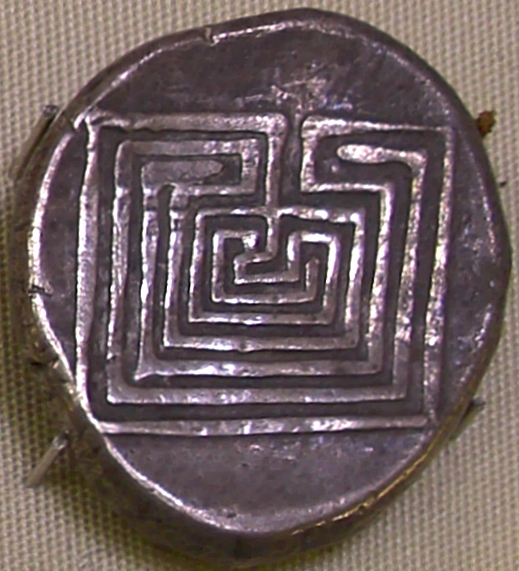
\includegraphics[width=0.3\textwidth]{images/pieceknossos.jpeg}
    \caption{Pièce d'argent représentant un labyrinthe unicursal, 400 avant J.C. - AlMare - CC-BY-SA-3}
\end{figure}

Ainsi, les labyrinthes que nous connaissons n'ont réellement fait leur apparition qu'au XVI\textsuperscript{e} siècle\cite{McCullough2004}, en tant que jeu de réflexion et de divertissement.

\section{Labyrinthes et informatique}

Aujourd'hui, on retrouve de nombreuses installations permettant d'évoluer dans des labyrinthes, souvent végétaux (Haies, Maïs, etc.). Le labyrinthe est devenu un symbole de réflexion, de concentration et de patience, et est souvent utilisé dans des jeux vidéos, des films, des livres, etc.

Cette notion a notamment pris une dimension toute particulière dans les domaines des mathématiques et plus tard, de l'informatique. En effet, un labyrinthe peut être vu comme un graphe, où chaque case est un nœud et chaque passage entre deux cases est une arête.

Ainsi, utiliser un labyrinthe est un excellent moyen d'en apprendre plus sur les algorithmes de recherche, qui sont indispensables à d'innombrables technologies que nous utilisons aujourd'hui : les jeux vidéos, les applications de navigation, les moteurs de recherche, les intelligences artificielles, etc.

De nombreux problèmes mathématiques bien connus sont d'ailleurs basés sur la théorie des graphes et donc sur les labyrinthes, comme le problème du cavalier (un cavalier doit visiter une unique fois chaque case d'un échiquier) ou celui des sept ponts de Königsberg, tous deux résolus par Euler dès le milieu du XVIII\textsuperscript{e} siècle\cite{Alexanderson2006}\cite{Euler1759}.

De la même façon que les labyrinthes ont été utilisés afin d'étudier la mémoire chez les rats, des compétitions de résolution de labyrinthes sont organisées chaque année, notamment par la société américaine \textit{Micromouse}, qui propose aux participants de créer un robot capable de résoudre un labyrinthe en un temps record, sans aucune connaissance préalable du tracé du labyrinthe.\cite{Veritasium2023}

\section{Algorithmes de génération et de résolution de labyrinthes}

\subsection{Génération de labyrinthes}

\subsubsection{Un peu de théorie}

Afin de générer un labyrinthe, il peut être très utile d'en apporter une définition mathématique plus rigoureuse.

Si on choisit l'approche de la théorie des graphes, alors un labyrinthe peut être décrit comme un graphe grille : un graphe non orienté où chaque nœud est relié à ses quatre voisins (haut, bas, gauche, droite) s'ils existent.

Chaque nœud représente un chemin du labyrinthe, et chaque arête représente le passage d'une case à une autre. Certaines propriétés intéressantes sont déjà présentes : on ne peut par exemple pas se déplacer d'une case à une autre si elles ne sont pas adjacentes, c'est à dire reliées par une arête.

Pour ajouter le concept de mur au labyrinthe, il suffit de retirer la connexion entre deux nœuds pour ajouter un "obstacle virtuel" entre les cases, empêchant ainsi le passage.

À partir de cette définition, on peut considérer que n'importe quel graphe ainsi dérivé d'un graphe grille, avec un nombre arbitraire d'arêtes manquantes, est un labyrinthe. Toutefois, afin de rendre les choses plus intéressantes, il est bon de rajouter quelques contraintes.

Il peut par exemple être intéressant de nécessiter l'existence d'au moins un chemin entre n'importe quelle case de départ, et n'importe quelle case d'arrivée. Cette contrainte est appelée la connexité du graphe, et est souvent utilisée pour garantir qu'un labyrinthe est "solvable".

On peut également pousser le vice et exiger que le chemin qui relie deux cases du labyrinthe soit unique. Si on considère notre graphe grille, alors un tel labyrinthe serait représenté par un arbre, c'est à dire un graphe convexe et acyclique (il est impossible de partir d'un sommet et d'y revenir sans rebrousser chemin au moins une fois). Plus encore, il s'agit d'un arbre couvrant, puisqu'il couvre l'ensemble des sommets du graphe de départ.

Dans ce contexte, un labyrinthe qui vérifie ces deux conditions est appelé un labyrinthe parfait. Ainsi, la plupart des algorithmes de génération ont été conçus pour produire des labyrinthes parfaits.

Toutefois, il est très souvent plus intéressant de travailler avec des labyrinthes non-parfaits, et où plusieurs chemins sont possibles. On peut ainsi tester les algorithmes de résolution sur un critère supplémentaire : la longueur du chemin trouvé, que l'on précisera dans la suite de cette partie.

Parallèlement, un algorithme de génération de labyrinthe peut être comparé sur la base de deux critères : le temps de génération, ainsi que la "difficulté" du labyrinthe généré, ce qui est assez peu objectif.

\subsubsection{L'algorithme "Depth-first search"}

Dans le cadre de ce projet, nous avons choisi de générer des labyrinthes en utilisant l'algorithme de \textit{depth-first search}, également appelé \textit{recursive backtracking}, un algorithme de type "diviser pour régner" qui consiste à diviser le problème en sous-problèmes plus petits, les résoudre, puis les combiner pour obtenir la solution du problème initial.

Malgré son nom, son implémentation ne nécéssite pas d'utiliser une récursion au sens strict, et est souvent plus performante de façon itérative, en utilisant une \textbf{pile} pour stocker les états précédents. L'utilisation d'une pile, en plus d'être plus sûre (en évitant d'éventuells erreurs liées à un manque de mémoire dans la pile d'appel des fonctions), permet de faciliter la visualisation de l'algorithme, en rendant accessibles toutes les données qui y sont liées à tout moment.

L'algorithme fonctionne de la façon suivante :

\begin{enumerate}
    \item On considère un labyrinthe où chaque case est entourée par des murs. On définit une pile vide.
    \item Choisir un point de départ dans le labyrinthe.
    \item Marquer ce point comme visité et l'ajouter à la pile.
    \item Tant qu'il existe des voisins non visités :
          \begin{enumerate}
              \item Retirer la case en haut de la pile et la définir comme la "case courante"
              \item Si la case courante possède au moins un voisin qui n'a pas été visité :
                    \begin{enumerate}
                        \item Ajouter la case courante à la pile
                        \item Choisir un de ses voisins non visités (aléatoirement)
                        \item Retirer le mur entre la case courante et le voisin choisi
                        \item Marquer le voisin comme visité et l'ajouter à la pile
                    \end{enumerate}
          \end{enumerate}
\end{enumerate}

Cet algorithme garantit la génération d'un labyrinthe parfait. De plus, il est relativement simple à implémenter et produit des labyrinthes avec une structure intéressante.

Après considération des alternatives existantes, nous avons jugé que l'intérêt d'implémenter d'autres algorithmes de génération de labyrinthes n'était pas suffisant pour justifier le temps et les ressources nécessaires à leur implémentation. En effet, les alternatives existantes telles que les algorithmes de Kruskal ou de Prim ne présentent pas d'avantages significatifs ou de résultats significativement différents par rapport à l'algorithme de \textit{depth-first search}.

La principale différence entre les labyrinthes générés par ces algorithmes réside dans sa structure : le \textit{depth-first search} génère des labyrinthes avec de longs couloirs, tandis que les algorithmes de Kruskal et de Prim génèrent des labyrinthes avec des couloirs plus courts, rendant une grande partie du labyrinthe fondamentalement inutile du point de vue de la résolution.

Afin d'ajouter de la diversité à nos labyrinthes, et de rendre le processus de résolution beaucoup plus intéressant, nous avons décider d'implémenter ce que nous avons appelé un "facteur de bouclage" : il s'agit d'un réel compris entre $0$ et $1$, et qui permet de transformer un labyrinthe parfait en labyrinthe comportant de nombreux chemins différents entre deux cases.

Une fois un labyrinthe généré, on sélectionne aléatoirement un certain nombre de murs en fonction du facteur de bouclage (un facteur de $0.5$ signifiant que la moitié des murs du labyrinthe seront retirés), et on les retire du labyrinthe. On obtient ainsi un labyrinthe non-parfait, mais toujours solvable.

\subsection{Résolution de labyrinthes}

\subsubsection{Un peu de théorie}

L'élucidation d'un labyrinthe consiste principalement en la recherche d'un chemin dans un graphe, tout en tenant compte des propriétés spécifiques de ce dernier, comme abordé précédemment.

Ainsi, il est tout à fait possible d'utiliser n'importe quel algorithme de recherche de chemin dans un graphe pour résoudre n'importe quel labyrinthe, comme par exemple l'algorithme de Dijkstra.

Toutefois, le contexte du labyrinthe permet également de rajouter certaines contraintes optionnelles à la résolution, comme par exemple le fait de se mettre à la place d'un joueur ne pouvant pas voir l'ensemble du labyrinthe à la fois. De plus, certains algorithmes ne fonctionnent que sur des arbres couvrants, c'est à dire des labyrinthes parfaits.

On peut citer par exemple deux algorithmes triviaux de résolution de labyrinthes : le mur suiveur, qui consiste à suivre un mur à sa droite ou à sa gauche jusqu'à trouver la sortie, et celui de la "souris aléatoire", qui consiste à se déplacer aléatoirement dans le labyrinthe jusqu'à trouver la sortie.

Ce dernier algorithme est d'ailleurs plus intéressant qu'il en a l'air : il est évidemment très peu performant, mais c'est un exemple d'\textit{algorithme de Las Vegas}, c'est à dire un algorithme aléatoire qui est garanti de trouver une solution correcte au problème qui lui est présenté.

De son côté l'algorithme de mur suiveur fonctionne uniquement sur des labyrinthes parfaits, et peut rentrer dans des boucles infinies si ce n'est pas le cas.

Comme nos labyrinthes ne sont pas parfaits, et que l'objectif reste d'en trouver une solution dans un temps raisonnable, nous avons choisi d'implémenter deux algorithmes beaucoup plus performants que ceux-ci : \texttt{recursive backtracking} et \texttt{A*}.

\subsubsection{L'algorithme "Recursive backtracking"}

L'algorithme \texttt{recursive backtracking} est un algorithme qui consiste à identifier les impasses du labyrinthes, et de les "bannir" afin de ne plus les emprunter. Cet algorithme est bien le même que celui qui permet de générer des labyrinthes, mais en sens inverse. Il porte donc le même nom, mais afin d'éviter toute confusion, nous avons fait le choix de l'appeler exclusivement "\textit{recursive backtracking}", tandis que l'algorithme de génération est appelé "\textit{depth-first search}".

Bien que sur le papier, il soit similaire à celui que nous avons déjà étudié, il est en réalité légèrement différent dans son implémentation. En plus de la pile et de la liste de cases déjà visitées, on va également utiliser une liste de cases bannies, qui sont des cases qui ne mènent à aucune solution.

L'algorithme fonctionne de la façon suivante :

\begin{enumerate}
    \item On considère un labyrinthe quelconque, avec une case de départ et une case d'arrivée. On initialise une pile contenant la case de départ, une liste de cases déjà visitées vide, et une liste de cases bannies vide.
    \item Tant que la pile ne contient pas la case d'arrivée :
          \begin{enumerate}
              \item On choisit une case voisine non visitée, non bannie, et non séparée par un mur de la case en haut de la pile.
              \item Si aucune case n'est disponible, on retire la case en haut de la pile et on l'ajoute à la liste de cases bannies.
              \item Sinon, on ajoute la case choisie à la pile et on la marque comme visitée.
          \end{enumerate}

    \item Lorsque la pile contient la case d'arrivée, on a trouvé une solution : la pile contient le chemin entre la case de départ et la case d'arrivée.
\end{enumerate}

Cet algorithme est raisonnablement performant, mais n'est pas nécessairement garanti de trouver le chemin le plus court entre deux cases. Il est toutefois garanti de trouver une solution si elle existe.

\subsubsection{L'algorithme "A*"}

L'algorithme \texttt{A*} est un algorithme de recherche de chemin dans un graphe qui utilise une heuristique pour guider la recherche. Il est souvent utilisé dans des contextes où la recherche de chemin est difficile, comme par exemple dans les jeux vidéos, les applications de navigation, etc.

Une heuristique est une fonction qui permet de "guider" l'algorithme dans ses choix en faisant des hypothèses jugées "raisonnables". Par exemple, dans l'algorithme précédent, lorsque plusieurs cases sont valides, on en choisit une au hasard. Ici, on fera appel à une fonction qui permettra de choisir la case la plus "prometteuse" parmi les cases valides.

Cette fonction peut grandement varier en fonction du contexte, par exemple en tenant compte du poids d'une connexion dans un graphe (la vitesse de circulation sur une route par exemple). Ici, on utilisera la distance de Manhattan, c'est à dire la somme des distances horizontales et verticales entre deux cases.

Comme l'algorithme est basé sur des hypothèses, il n'est également pas garanti de trouver une solution optimale. Toutefois, il trouve généralement des solutions qui s'en approchent en un temps très court. De plus, il est garanti de trouver une solution si elle existe.

Ses nombreux avantages et sa grande adaptabilité en font un algorithme très populaire : il est notamment utilisé par défaut dans de nombreux moteurs de jeux vidéos, et est souvent utilisé dans des compétitions de résolution de labyrinthes.

\subsubsection{D'autres algorithmes}

Il existe de très nombreux autres algorithmes de résolution de labyrinthe, ayant tous leurs avantages et inconvénients. On peut citer par exemple l'algorithme de Dijkstra, l'algorithme de Bellman-Ford, l'algorithme de Floyd-Warshall, etc.

Bien que leur implémentation ne soit pas nécéssairement plus complexe que celle des algorithmes que nous avons choisi d'implémenter, nous avons préféré passer plus de temps à créer des visualisations et des fonctionnalités supplémentaires pour le programme plutôt que d'implémenter de nouveaux algorithmes.

L'ajout de ces algorithmes pourrait être une piste d'améliorations pour le futur, comme il le sera précisé dans le cinquième et dernier chapitre de ce rapport.

\chapter{Méthodologie}


Au sein de ce chapitre, nous allons décrire les différentes étapes de développement du programme, en décrivant les outils utilisés ainsi que les différentes étapes de conception.

Il est bon de rappeler que des instructions détaillées sur l'installation du programme et la consultation du code source sont disponibles en annexe 1. Il est également possible de consulter directement le dépôt Git du projet à l'adresse suivante : \url{https://github.com/HerbeMalveillante/ProjetPeiP24}

\section{Versionnage}

Garder une trace de l'évolution du code source est une étape cruciale dans tout projet informatique, surtoût lorsqu'il est réalisé en équipe.

Conserver le projet stocké en "local" sur une machine est la meilleure façon de s'exposer à des pertes de données, des erreurs de manipulation, etc. De plus, il est souvent nécessaire de travailler en même temps sur un même fichier, ce qui peut être une source de conflits évidente.

Imaginons que deux développeurs modifient le même fichier en même temps, et que l'un des deux enregistre ses modifications avant l'autre. Lorsque le second enregistre ses modifications, il écrase celles du premier, et les modifications de ce dernier sont perdues. C'est ce qu'on appelle un conflit.

De plus, si un changement majeur dans le code source provoque un bug et qu'il est difficile de faire machine arrière, il est souvent nécessaire de revenir à une version antérieure du code source, ce qui peut faire perdre beaucoup de progression si les sauvegardes n'ont pas été régulières.

Pour éviter tous ces problèmes, il est nécessaire d'utiliser un logiciel de gestion de version, qui permet de conserver un historique de toutes les modifications apportées au code source, de revenir à une version antérieure, de créer des branches pour travailler sur des fonctionnalités différentes, etc.

L'outil que nous avons choisi d'utiliser est Git\cite{Git2024}, associé à la plateforme en ligne GitHub\cite{GitHub2024}.

\subsection{Git}

Git est un logiciel libre de gestion de version créé par Linus Torvalds (le créateur du noyau Linux) en 2005. Il est aujourd'hui le logiciel de ce type le plus utilisé au monde, et est considéré comme un standard de facto dans le monde du développement logiciel de part sa nature libre et gratuite, et sa grande robustesse.

Git peut fonctionner de façon décentralisée, c'est à dire que chaque développeur peut avoir une copie du code source sur sa machine, et travailler dessus de façon indépendante. Il est également possible de travailler en équipe, en partageant le code source sur un serveur distant, et en synchronisant les modifications apportées par chaque développeur.

Lorsqu'on a terminé une fonctionnalité, on peut "commit" nos modifications, c'est à dire les enregistrer dans l'historique du projet. On peut ensuite "push" ces modifications sur le serveur distant, où elles seront visibles par les autres membres de l'équipe qui pourront les "pull" pour les télécharger sur leur machine.

Si des conflits surviennent, Git est capable de les gérer de façon très efficace, en permettant de les résoudre manuellement, ou en utilisant des outils de résolution de conflits.

Cet outil est également très utile pour travailler collaborativement grâce à son système de branches, qui permet de travailler sur des fonctionnalités différentes en parallèle, et de fusionner ces branches une fois les fonctionnalités terminées afin d'éviter de mettre en ligne des fonctionnalités non abouties sur la branche principale.

Git est disponible sous forme de ligne de commande, mais il existe également de nombreuses interfaces graphiques qui permettent de l'utiliser de façon plus intuitive.

\subsection{GitHub}

GitHub est une plateforme en ligne qui fait office de serveur distant pour les projets Git. Elle permet d'héberger des projets gratuitement afin de les rendre accessibles à tous facilement et est ainsi le berceau de nombreux projets open-source tels que le noyau Linux lui-même\cite{LinuxGithub2024}, le langage de programmation Python\cite{PythonGithub2024}, etc.

En plus de cette fonctionnalité, GitHub propose de nombreux outils supplémentaires pour faciliter la coopération et permettre à des collaborateurs externes de facilement travailler sur un projet, en créant sa propre "version alternative" appelée "fork", en proposant des modifications au projet original appelées "pull requests", en faisant des rapports de bugs, etc.

Parfois, certaines versions alternatives peuvent devenir aussi populaires que le projet original, comme c'est le cas de la version communautaire de Pygame, qui est utilisée pour ce projet.

Tout au long du projet, nous avons utilisé Git et GitHub pour conserver un historique de nos modifications, ce qui s'est avéré très utile. Nous avons également pu utiliser GitHub pour en mettre à disposition le code source.

\section{Programme principal}

\subsection{Langage de programmation, librairies et outils.}

Le langage de programmation que nous avons utilisé pour ce projet est Python, associé à la version communautaire de la librairie Pygame "Pygame-CE"\cite{PygameGithub2024}.

Le choix de cette librairie au lieu d'autres librairies graphiques a été basé sur sa simplicité d'utilisation, sa grande versatilité, ainsi que nos connaissances préalables avec cette librairie.

La version communautaire a été préférée pour ses nombreuses améliorations par rapport à la version officielle, notamment en termes de performances et de compatibilité avec les dernières versions de Python. En effet, la version originale de Pygame est de moins en moins maintenue. Les programmes écrits avec la version officielle fonctionnent correctement avec la version communautaire, mais l'inverse n'est pas garanti.

Des outils de formattage externe tels que \texttt{black}\cite{Black2024} ont également été utilisés pour garantir une cohérence dans le code source, et une conformité avec les standards \texttt{PEP 8}\cite{PEP82024} qui définissent les conventions en matière de style de code Python.

Les librairies \texttt{rich} et \texttt{graphviz} ont également été utilisées pendant le développement, la première pour améliorer la lisibilité des messages affichés dans la console (notamment lors de l'affichage de longs tableaux et listes), et la seconde lors de nos recherches sur les structures de données à utiliser pour stocker les labyrinthes. Ces librairies n'ont pas été utilisées dans la version finale du programme.

\subsection{Conception}

La première étape de la conception du programme a été de définir les différentes fonctionnalités que nous souhaitions implémenter, ainsi que de réaliser de nombreuses recherches sur les algorithmes de génération et de résolution de labyrinthes.

Nous avons ensuite défini une "liste de tâches" à réaliser, en les classant par ordre de priorité, avant de commencer à travailler sur des versions primitives du programme. Ces versions primitives nous ont permis de tester les algorithmes de génération et de résolution de labyrinthes, ainsi que de nous familiariser avec la librairie Pygame-CE et les diverses optimisations qu'il convient d'apporter pour obtenir les meilleures performances. Cette liste de tâches nous a également permis d'éclaircir les objectifs de la partie "libre" du projet, sur laquelle nous n'étions pas guidés par le sujet.

Un point majeur de cette étape fut de définir la structure de donnée à utiliser pour stocker les labyrinthes. En effet, il est tout à fait possible d'utiliser la programmation orientée objet pour définir un labyrinthe sous la forme d'un graphe, d'une matrice, d'une liste de cases, etc. L'enjeu était de trouver une structure adaptée aux algorithmes, mais également facile à utiliser pour l'adapter à l'interface graphique.

Une fois que nous avons obtenu des résultats satisfaisants et que nous avons défini une direction à suivre, nous avons pu commencer à travailler sur la version finale du programme, en ajoutant des fonctionnalités au fur et à mesure et en les testant régulièrement.

\section{Rédaction du rapport}

La rédaction du rapport a été réalisée en utilisant le langage de composition de documents \LaTeX (LaTeX), qui est un langage de balisage  avancé permettant de créer des documents de grande qualité typographique adaptés à la publication scientifique.

Ce langage est très populaire dans le monde de la recherche, et est souvent utilisé pour rédiger des articles, des thèses, des rapports, etc. Il permet de gérer de façon très efficace les références bibliographiques, les tableaux, les figures, les équations, etc.

Ainsi, nous avons pu nous concentrer sur le fond du rapport, LaTeX se chargeant automatiquement de la forme. Le code source du rapport est également disponible sur le dépôt Git du projet.

\chapter{Fonctionnalités}

Avant de d'expliquer l'implémentation et le fonctionnement du programme, il est utile de connaître les différentes fonctionnalités implémentées en son sein. Bien qu'il soit recommandé de tester le programme pour en avoir une idée plus précise, nous allons décrire les fonctionnalités du programme dans ce chapitre.

\section{Interface et éléments graphiques}

Afin de fournir à l'utilisateur une expérience agréable et intuitive, nous avons fait le choix de fournir une interface graphique permettant de contrôler la quasi-intégralité des paramètres du programme de façon visuelle, ainsi que d'accéder à toutes ses fonctionnalités.

Nous nous sommes inspirés du thème libre "Dracula"\cite{Dracula2024} pour les couleurs de l'interface, qui nous semble agréable à l'oeil et facile à lire. Nous avons opté pour des éléments interactifs minimalistes, que ce soit pour les boutons, les menus, les labyrinthes en eux-mêmes, les entités évoluant au sein du jeu, et même la police d'écriture.



\begin{figure}[h]
    \centering
    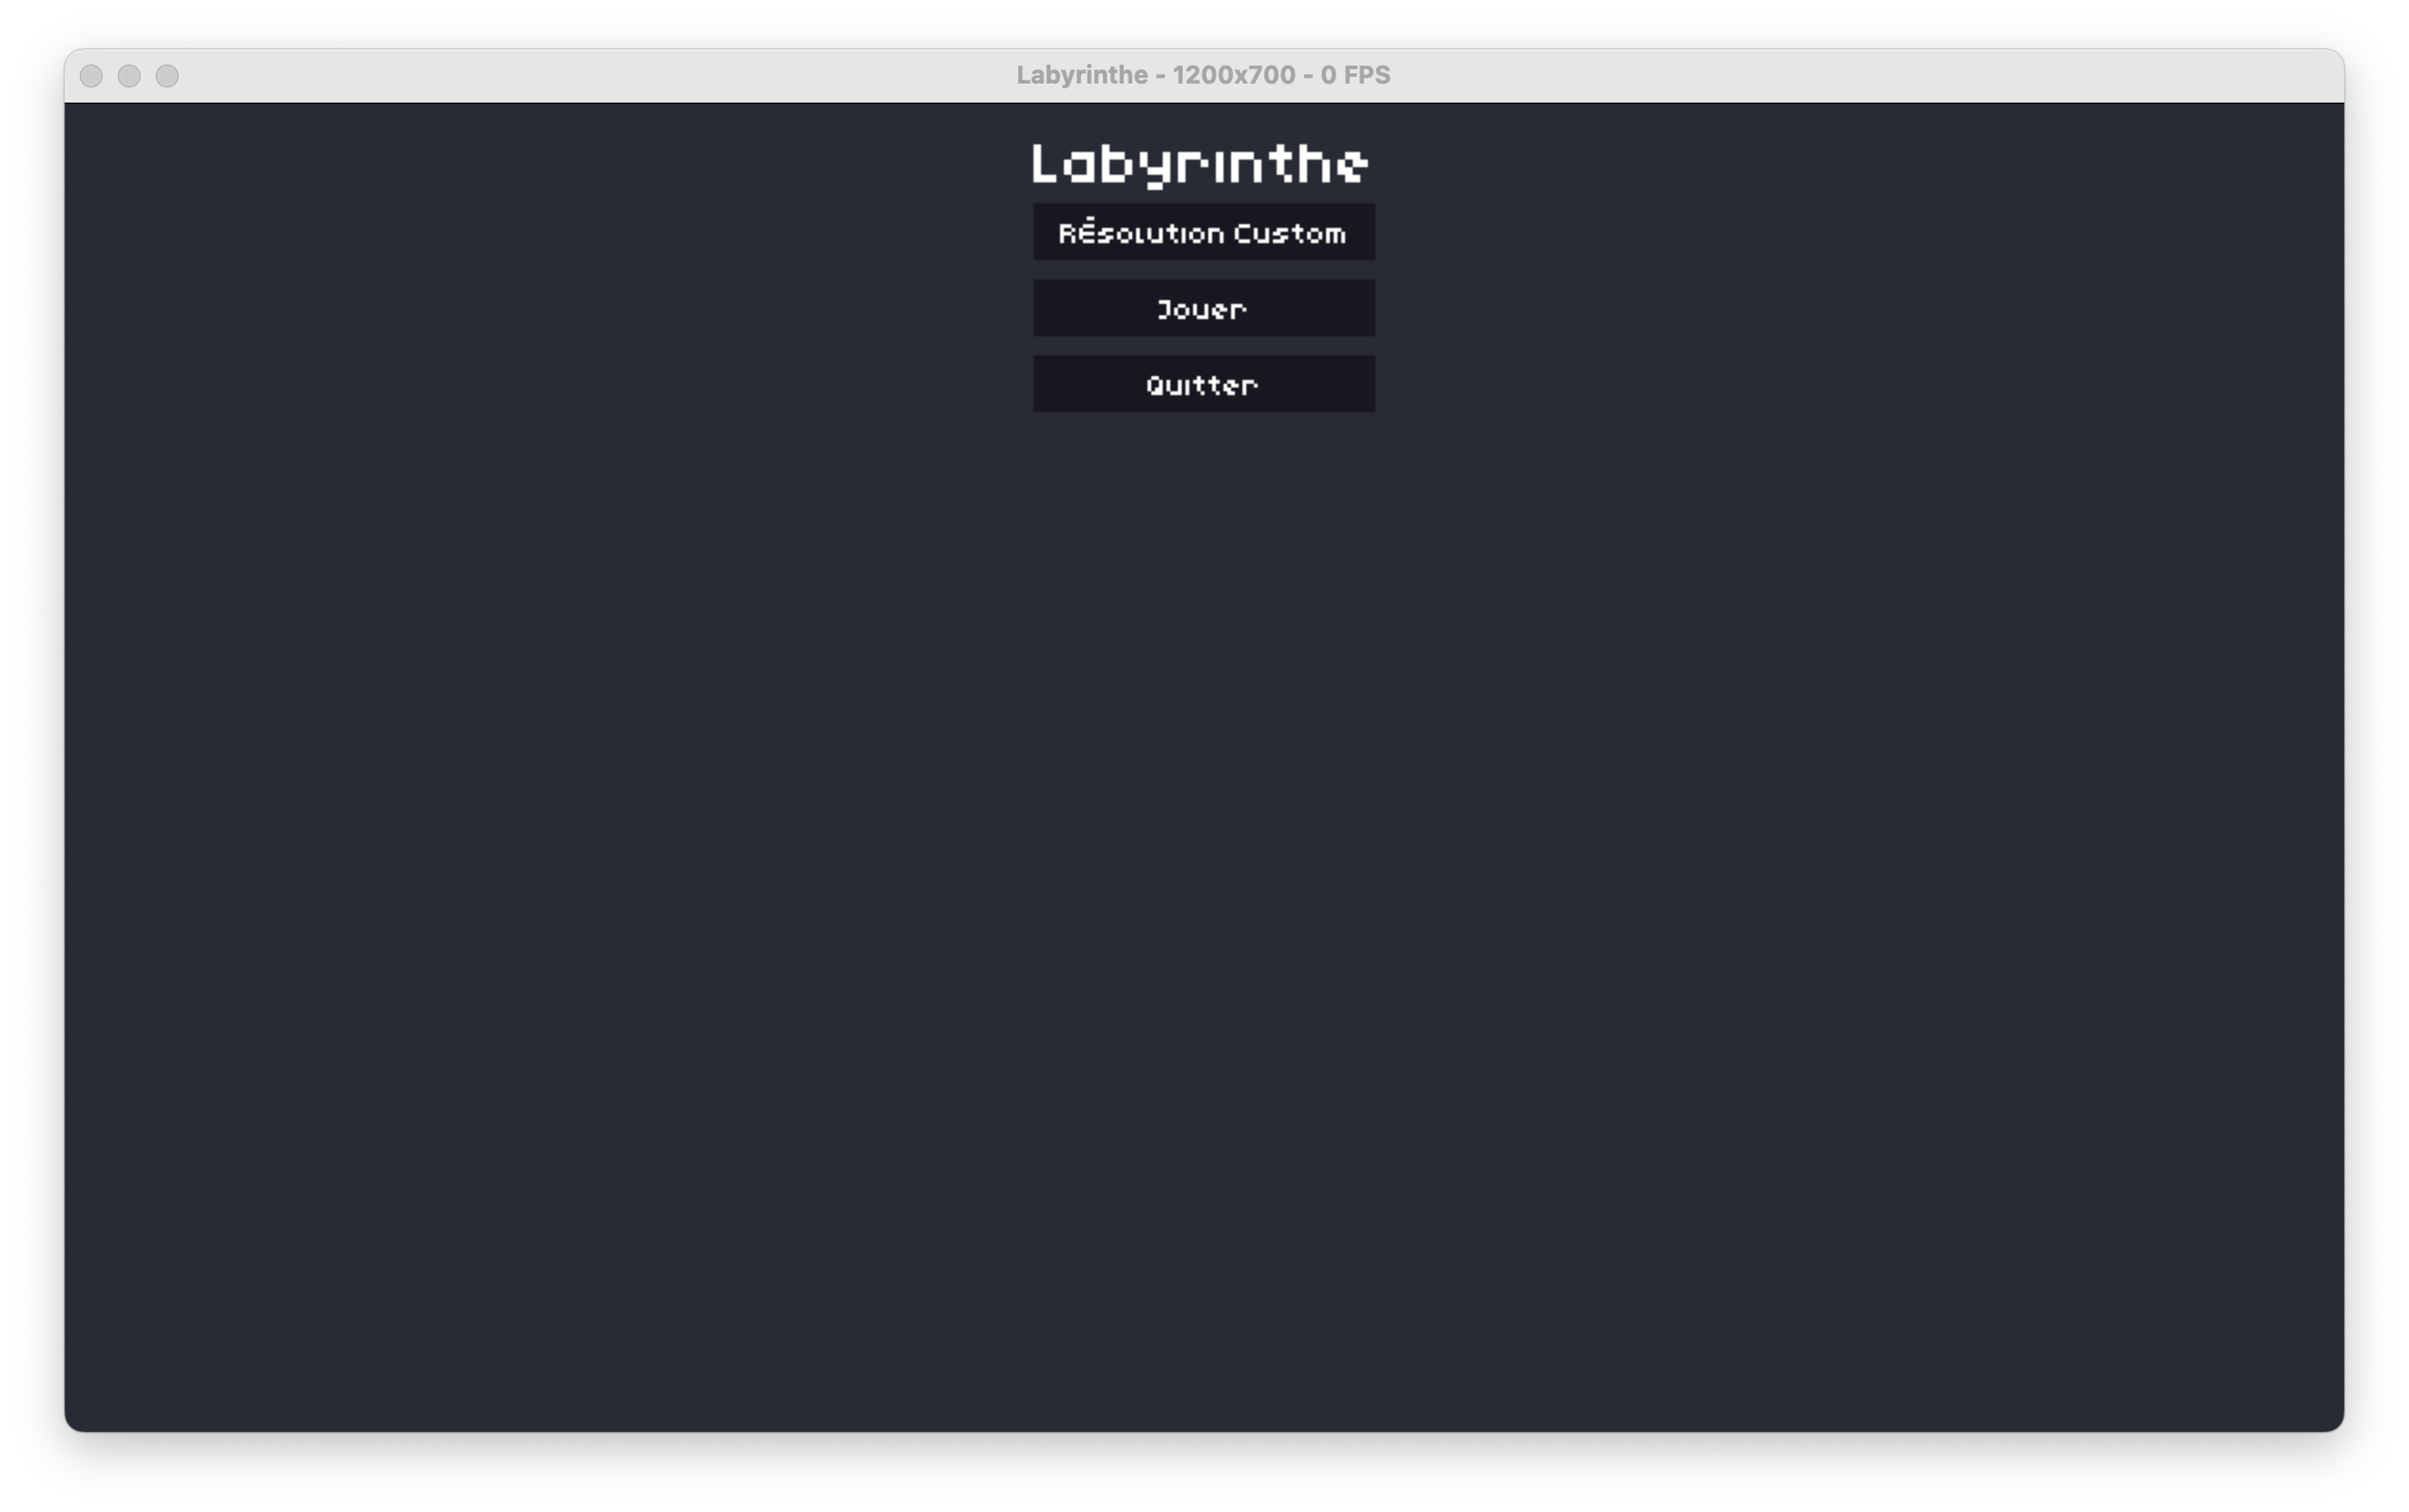
\includegraphics[width=\textwidth]{images/mainmenu.png}
    \caption{Capture d'écran du menu principal du programme}
\end{figure}

Tous les éléments graphiques sont générés à partir de classes réutilisables, garantissant une cohérence visuelle dans l'ensemble du programme. De plus, ces classes sont facilement modifiables, ce qui permet de changer l'apparence du programme en quelques lignes de code.

Des éléments permettant d'afficher du Texte dynamique (modifiable grâce à l'appel d'une méthode sur l'objet) et des Boutons interactifs permettant d'appeler une fonction ont été implémentés. Ces éléments sont personnalisables dans leur apparence et leur comportement.

Un système de navigation entre différents menus a été implémenté, permettant à l'utilisateur de naviguer facilement entre les différentes fonctionnalités du programme, tout en conservant les éventuelles informations déjà entrées lors d'un retour sur un écran précédent. De plus, aucune opération n'est bloquante, et l'utilisateur peut retourner en arrière à tout moment, même au beau milieu d'un algorithme.

Un système de cache des images a été mis en place afin de garantir une fréquence de rafraîchissement maximale en toutes circonstances, et un compteur d'images par seconde est visible dans la barre de titre de la fenêtre.

\section{Génération et résolution personnalisée}

Le premier menu disponible dans l'écran titre permet de générer un labyrinthe de taille personnalisée, et de le résoudre avec l'algorithme et le facteur de bouclage de son choix.

\begin{figure}[h]
    \centering
    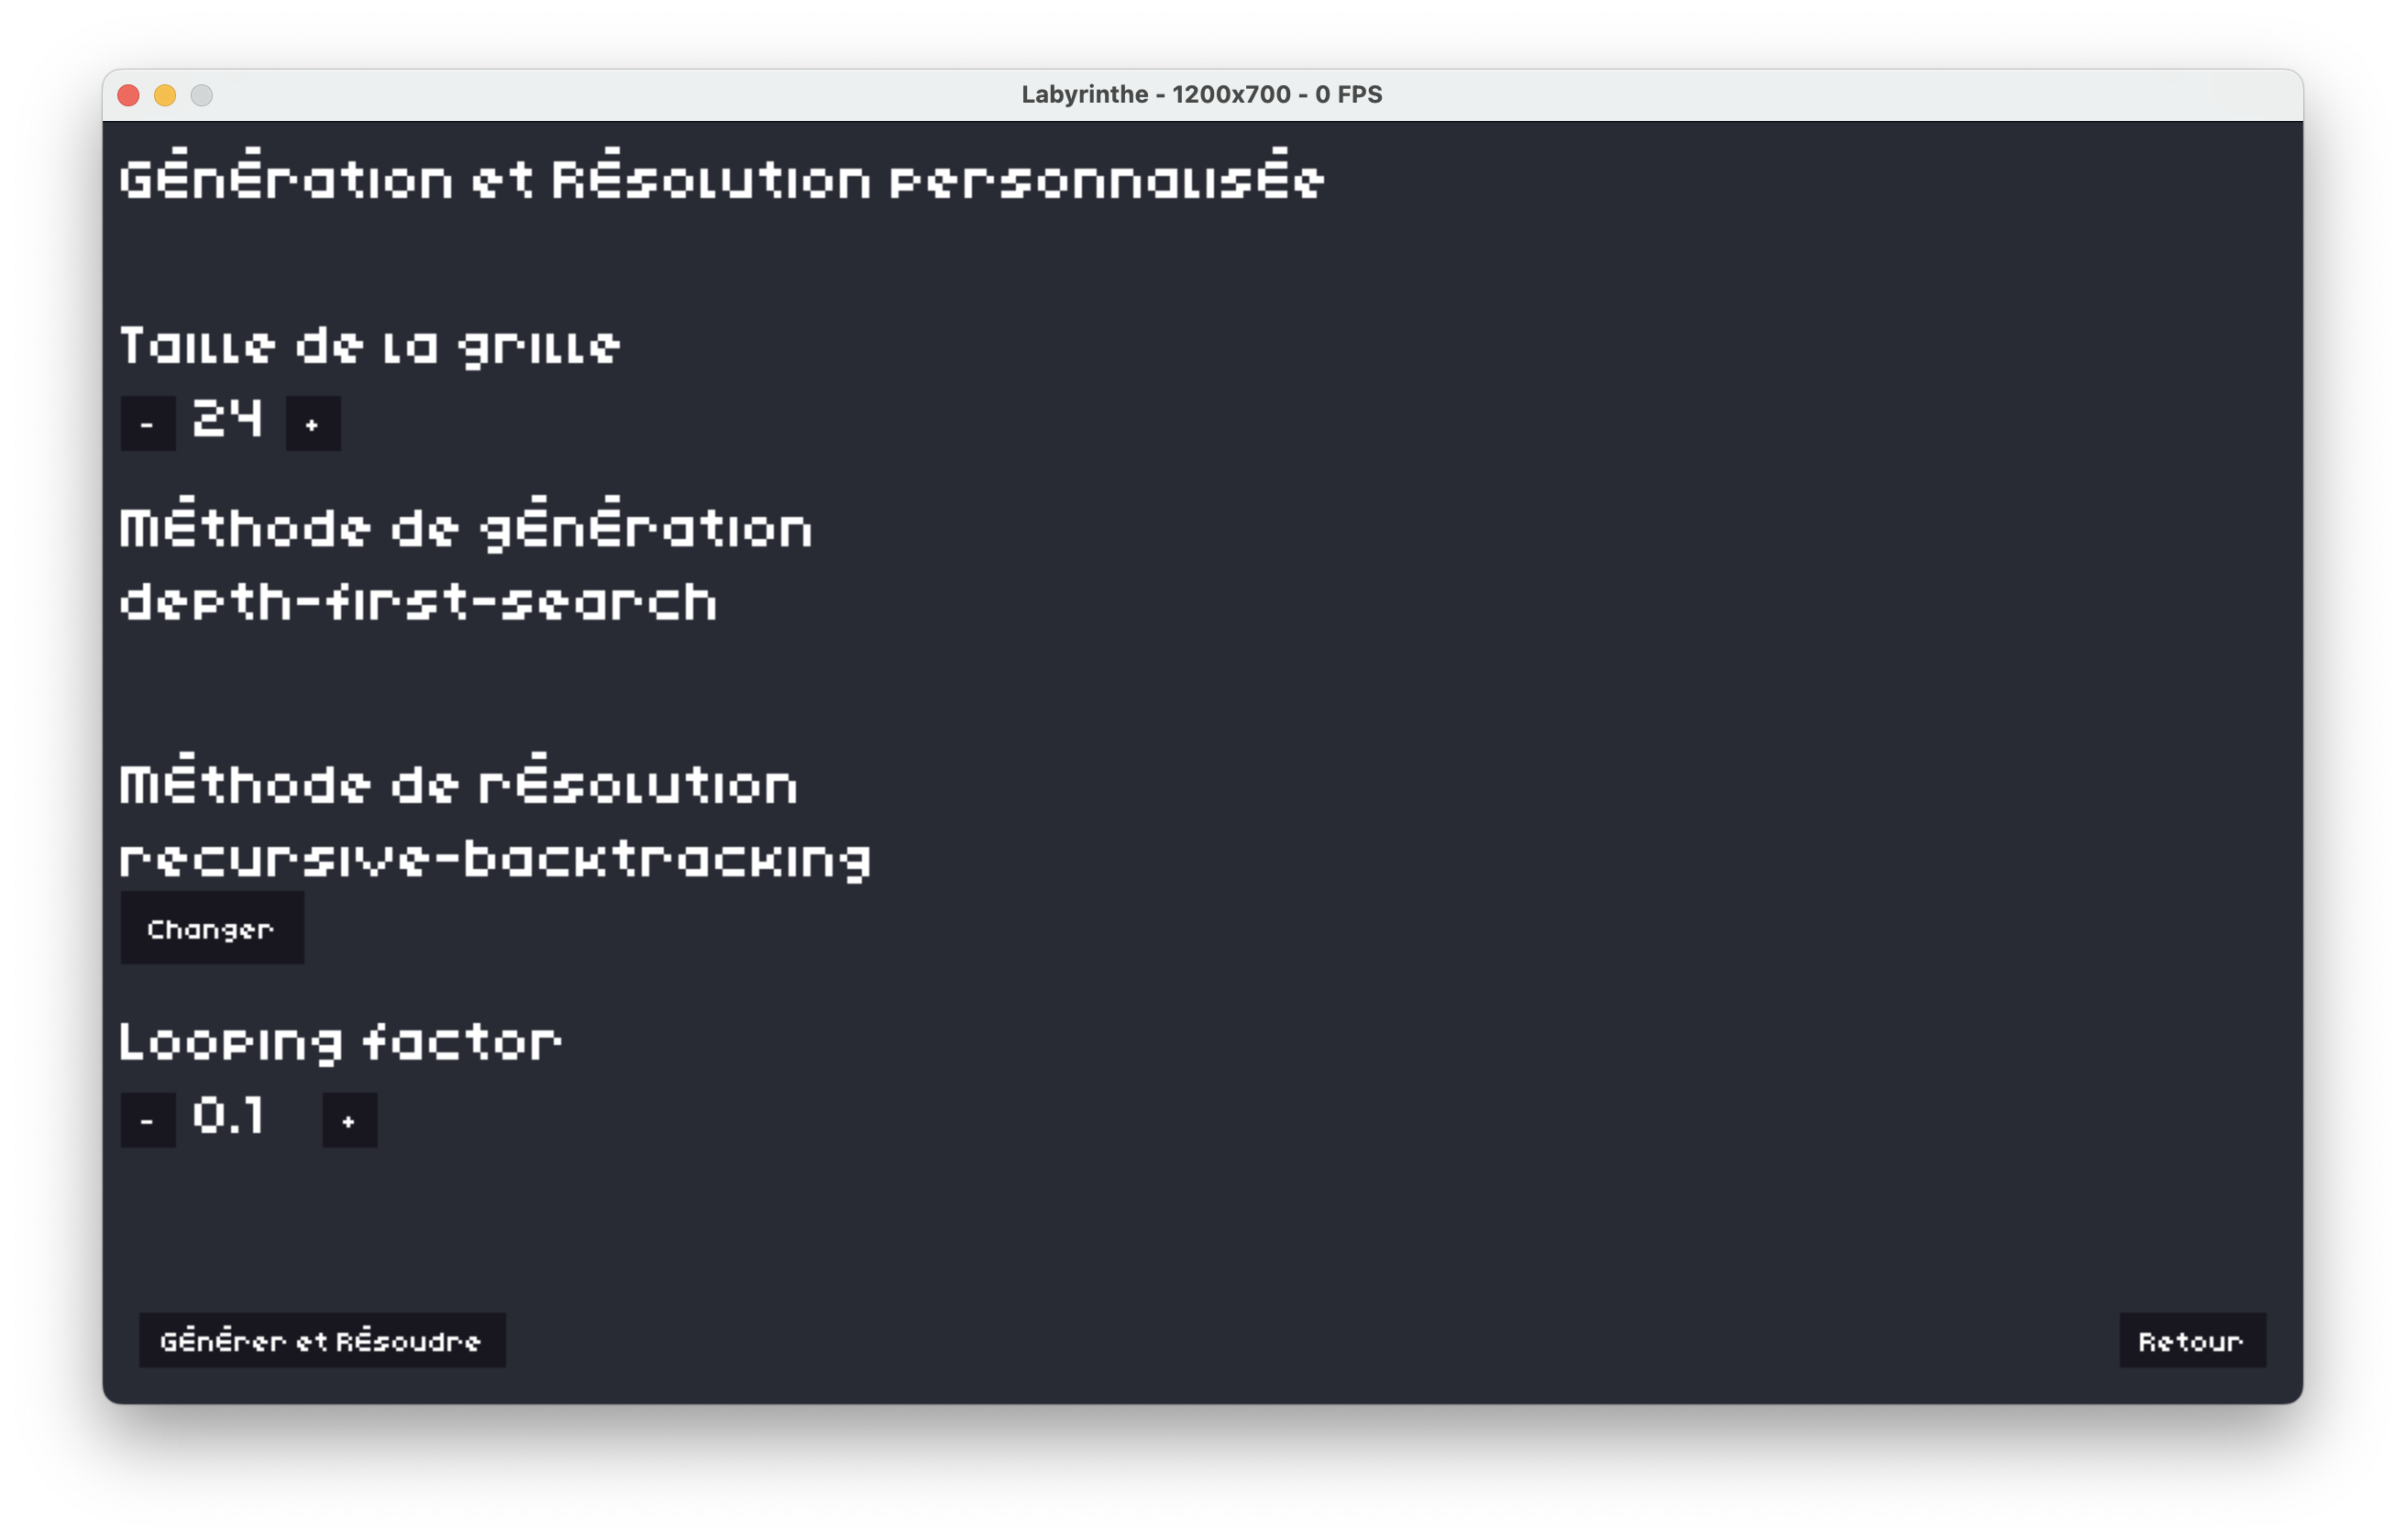
\includegraphics[width=\textwidth]{images/generationcustom.png}
    \caption{Capture d'écran du menu principal du programme}
\end{figure}

L'utilisateur peut choisir n'importe quelle taille supérieure à $2 \times 2$ (bien que des valeurs supérieures à 75 peuvent ne pas s'afficher correctement à l'écran en raison de la résolution limitée de ce dernier), et un facteur de bouclage compris entre $0.0$ et $1.0$ par pas de $0.05$. Un facteur de bouclage de $0.0$ résulte en un labyrinthe parfait, tandis qu'un facteur de bouclage de $1.0$ résulte en un labyrinthe où tous les murs ont été retirés.

Lorsque l'utilisateur clique sur "Générer et résoudre", le programme affiche une animation de la génération du labyrinthe, puis de sa résolution accompagnée de la visualisation appropriée. L'utilisateur peut à tout moment interrompre l'algorithme en cours en cliquant sur le bouton "Retour". L'ensemble des statistiques intéressantes sur la résolution sont visibles et mises à jour en direct sur la partie droite de l'écran.

L'algorithme de résolution commence en haut à gauche du labyrinthe, et cherche un chemin menant à la case en bas à droite.

\begin{figure}[h]
    \centering
    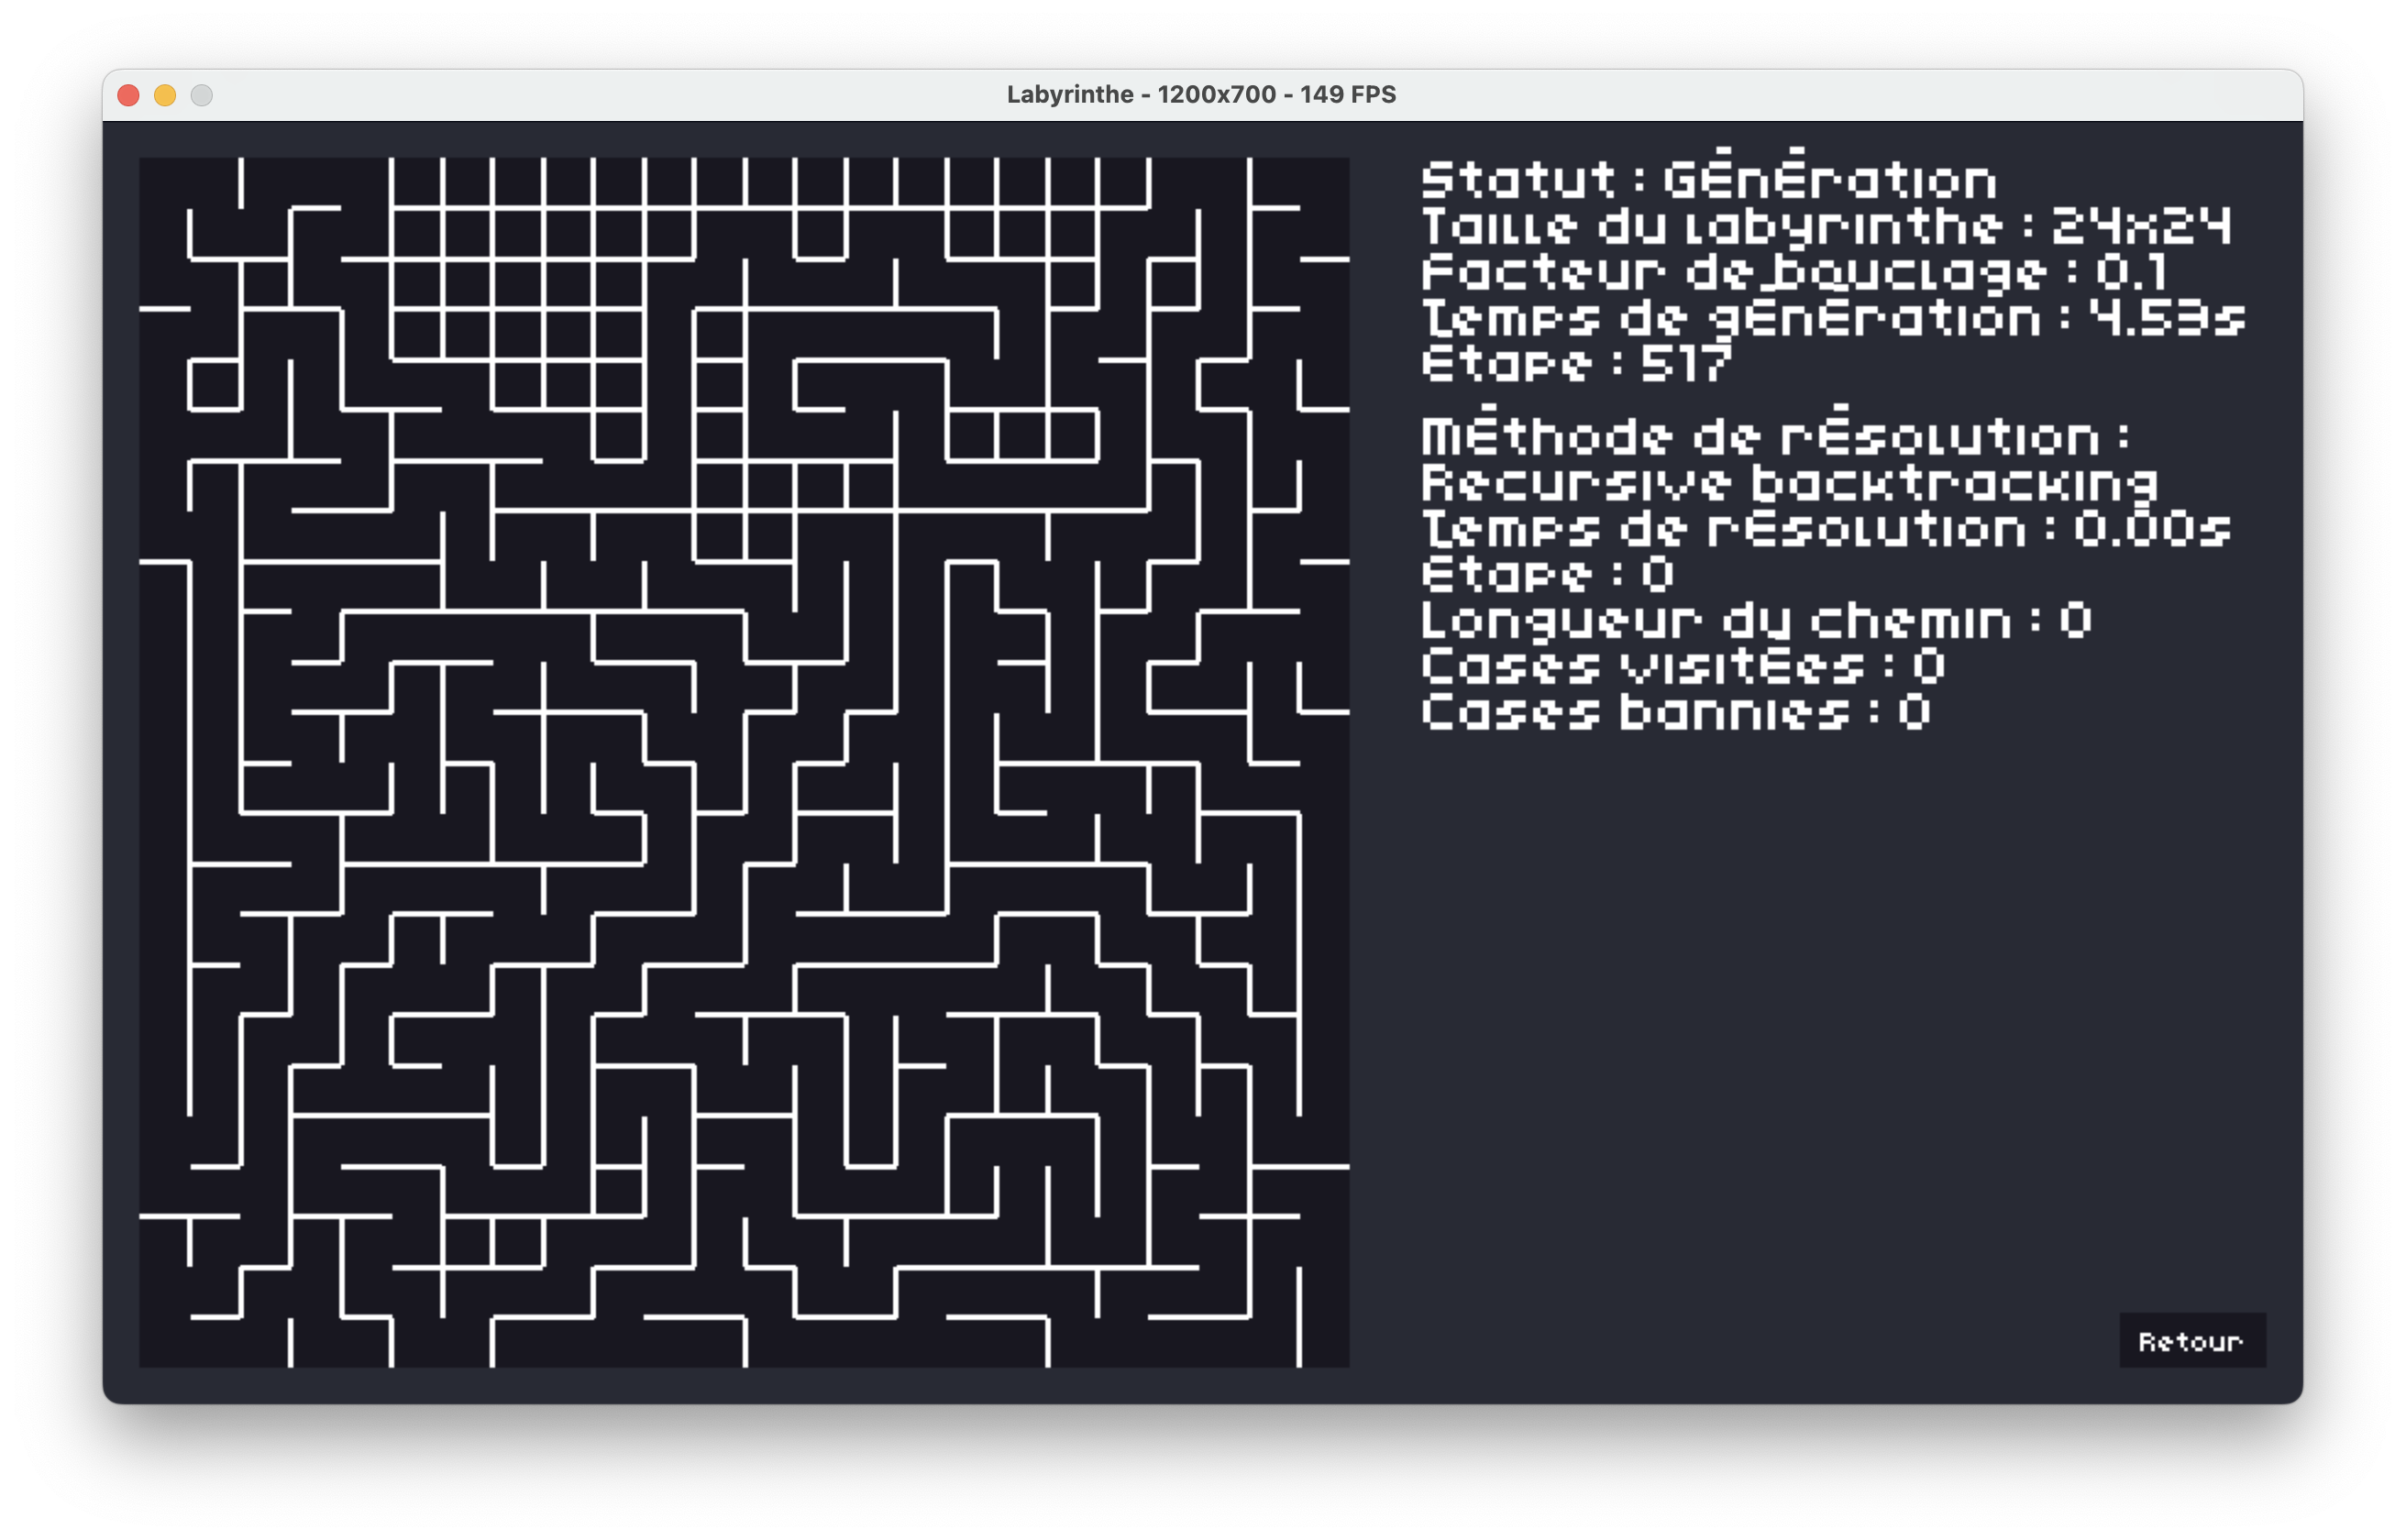
\includegraphics[width=0.70\textwidth]{images/labyrinthgeneratingsmall.png}
    \caption{Capture d'écran de la génération d'un labyrinthe de taille 24}
\end{figure}

\begin{figure}[h]
    \centering
    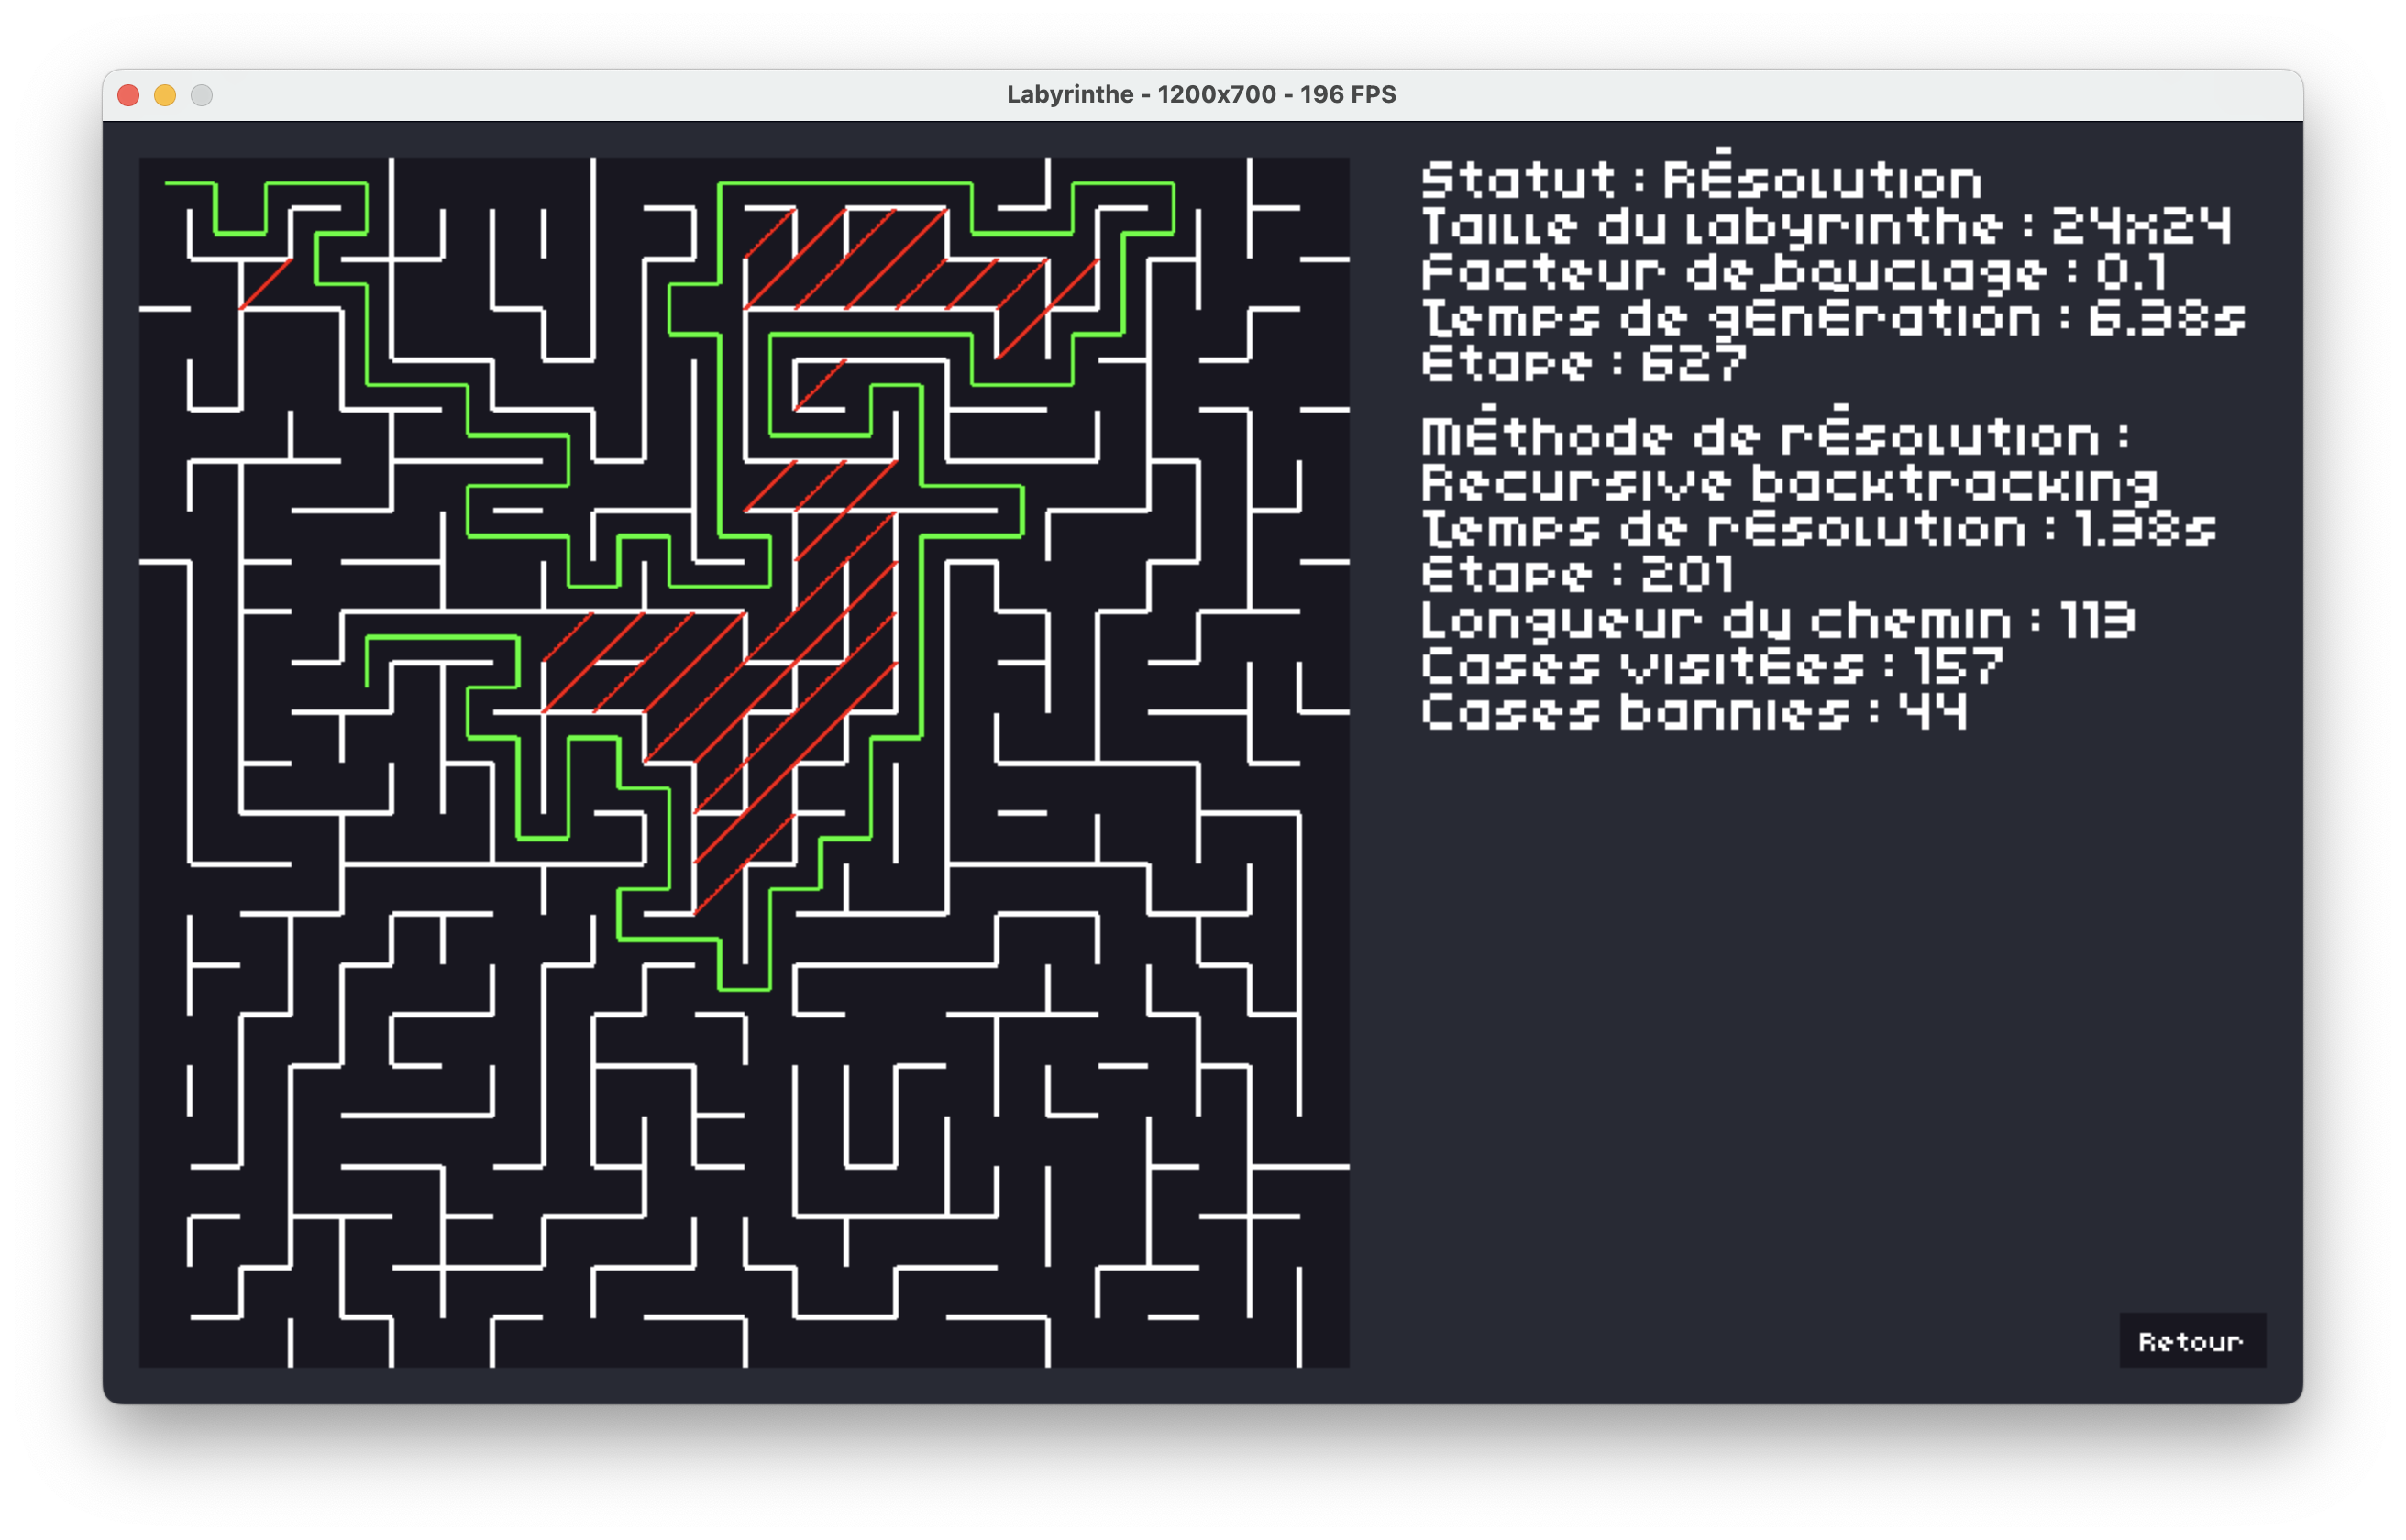
\includegraphics[width=0.70\textwidth]{images/recbacsolving24.png}
    \caption{Capture d'écran de la résolution d'un labyrinthe de taille 24}
\end{figure}


On observe sur ces images la génération et la résolution d'un labyrinthe de taille $24 \times 24$ avec un facteur de bouclage de $0.1$. On peut voir sur la droite de l'écran l'affichage de ces informations, ainsi que le temps et le nombre d'étapes de génération, ainsi que la méthode, le temps et le nombre d'étapes de résolution. Dans le cas de la résolution avec l'algorithme \texttt{recursive backtracking}, on peut également voir la longueur du chemin actuel, le nombre de cases visitées ainsi que le nombre de cases bannies.

On constate que la visualisation de cet algorithme consiste en l'affichage du chemin actuel en vert et des cases bannies barrées en rouge. On peut noter qu'il est inutile de signaler les cases visitées, qui sont soit également bannies soit sur le chemin actuel.

\begin{figure}[h]
    \centering
    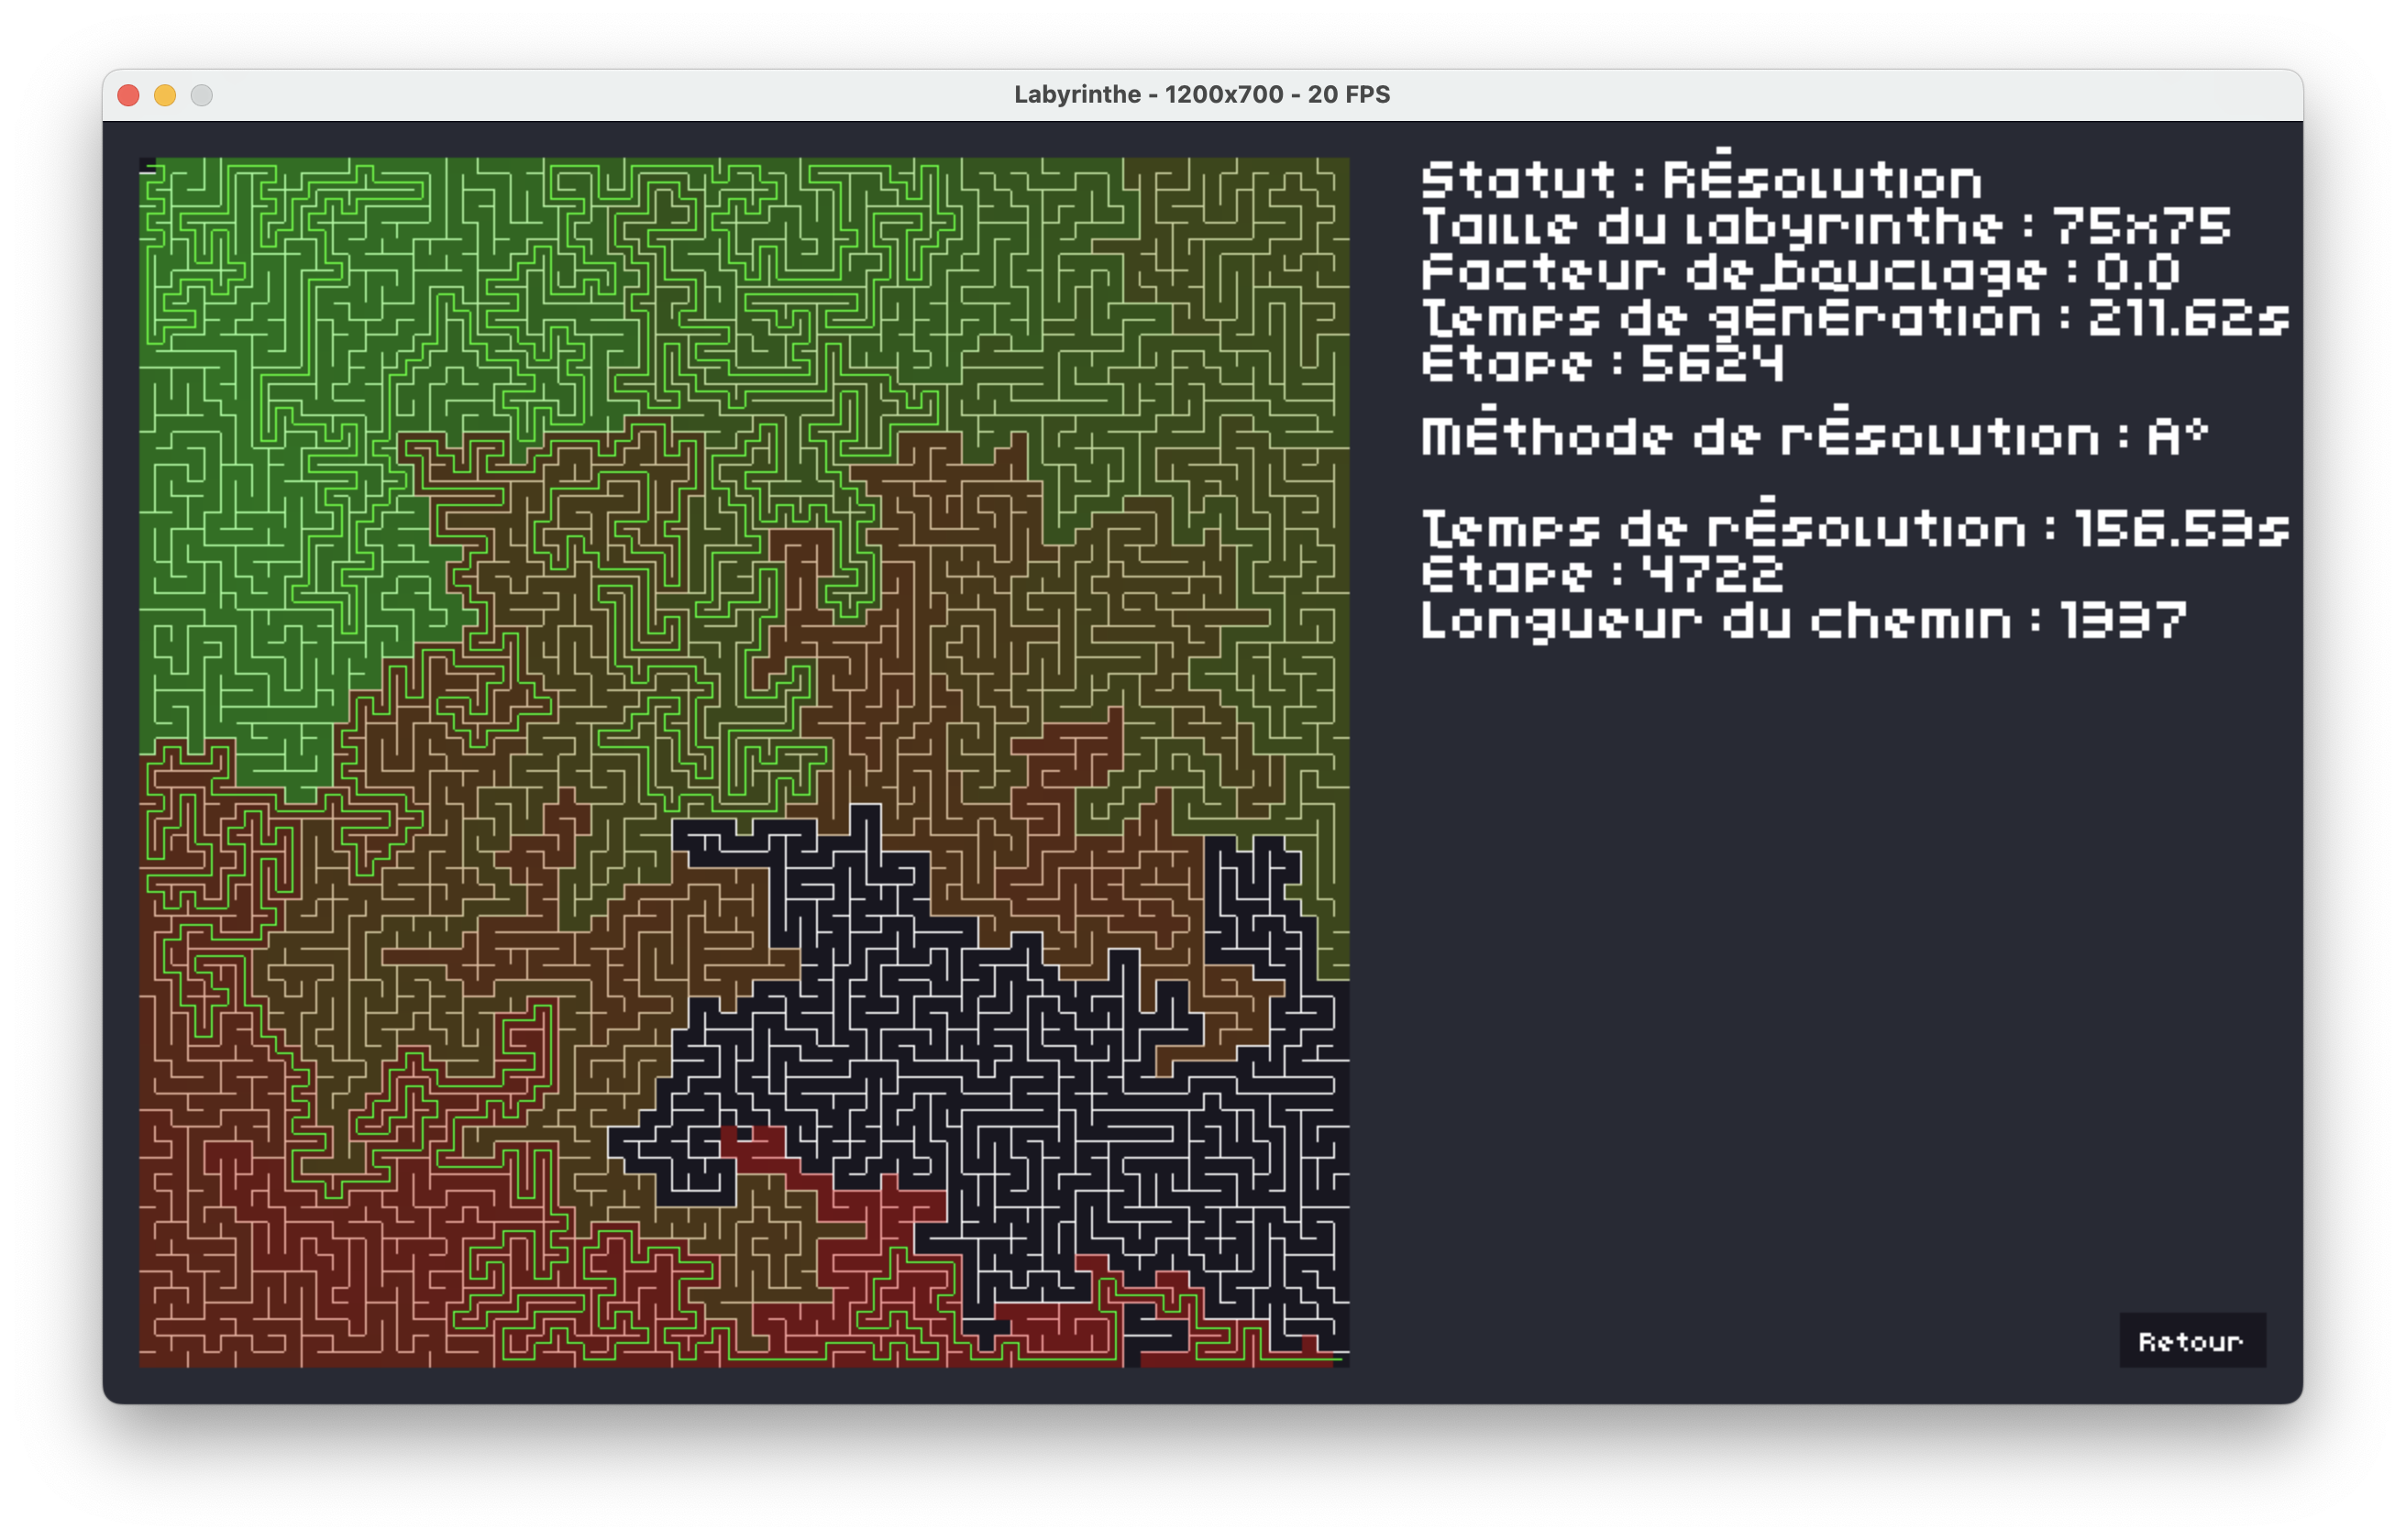
\includegraphics[width=\textwidth]{images/astarsolved75-2.png}
    \caption{Capture d'écran d'un labyrinthe parfait (facteur de bouclage de $0$) de taille $75 \times 75$ résolu avec l'algorithme \texttt{A*}}
\end{figure}

Sur cette capture d'écran, on peut voir un labyrinthe beaucoup plus grand ayant la particularité d'être parfait, c'est à dire que son facteur de bouclage vaut $0$ : il n'existe qu'un seul et unique chemin menant à l'arrivée.

Ces paramètres permettent à la fois de montrer un labyrinthe de grande taille, mais également la visualisation associée à l'algorithme \texttt{A*}, qui affiche non seulement le chemin actuel en vert, mais également le score individuel de chaque case sur un dégradé allant du vert au rouge : plus la case est verte, plus l'algorithme suppose qu'elle fait partie de la solution optimale.

\section{Résultats obtenus}

Les résultats obtenus par le programme sont très satisfaisants, et correspondent à nos attentes initiales. Les algorithmes de génération et de résolution fonctionnent correctement, et les labyrinthes générés sont variés et intéressants.

Il est également possible de comparer la performance des différents algorithmes : on constate sans vraiment de surprise que l'algorithme \texttt{A*} est beaucoup plus rapide que l'algorithme \texttt{recursive backtracking} quel que soit le facteur de bouclage.

Le temps de résolution n'étant pas un critère de performance utile étant donné qu'il dépend fortement de la fréquence de rafraîchissement et donc de la visualisation, il est plus intéressant de comparer le nombre d'étapes nécéssaires à la résolution, ainsi que la longueur du chemin trouvé. Dans les deux cas, l'algorithme \texttt{A*} est donc plus performant.


\begin{figure}[h]
    \centering
    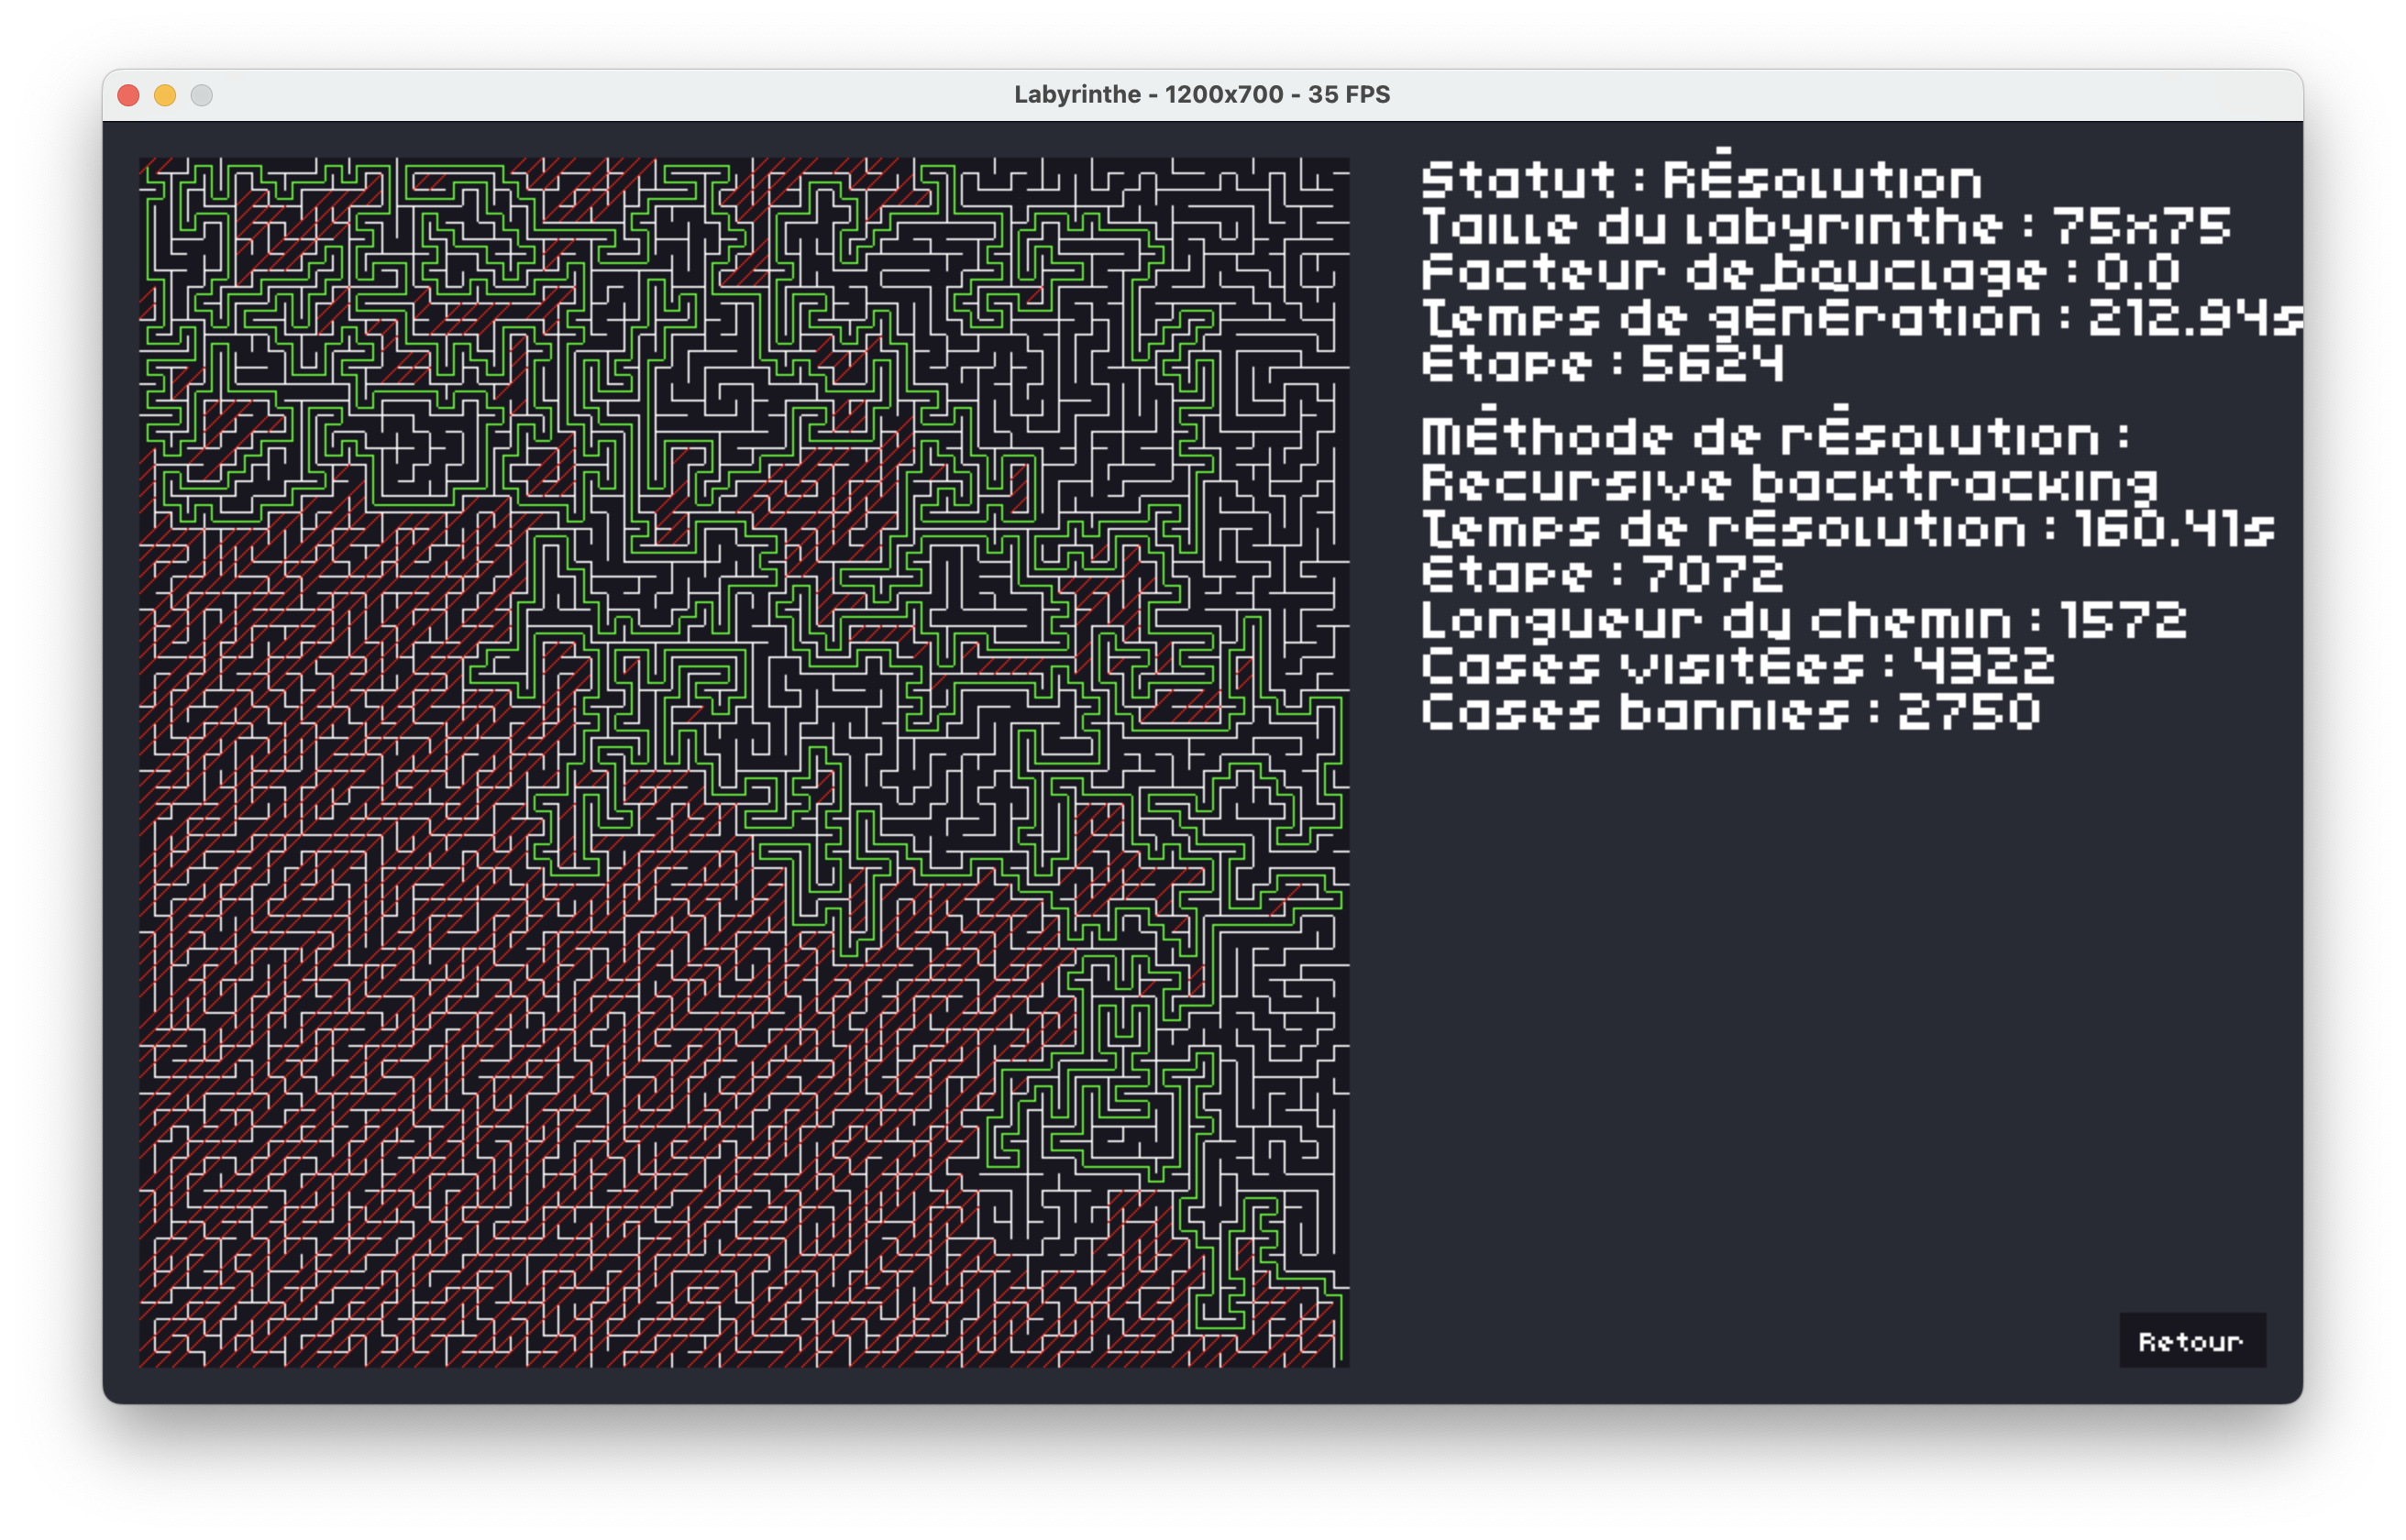
\includegraphics[width=\textwidth]{images/recbacksolved75.png}
    \caption{Capture d'écran d'un labyrinthe parfait (facteur de bouclage de $0$) de taille $75 \times 75$ résolu avec l'algorithme \texttt{recursive-backtracking}}
\end{figure}

Nous sommes également très satisfaits des performances du programme, qui descends rarement en dessous de 60 images par seconde, et uniquement lors de l'affichage de labyrinthes de très grande taille.

\section{Partie libre : création d'un jeu}

Une partie significative du projet était libre, et nous avons choisi de créer un petit jeu mettant à profit nos labyrinthes générés, ainsi que les algorithmes de résolution que nous avons implémentés.

Nous avons décidé de créer un jeu similaire au classique de l'arcade "PAC-MAN", où le joueur doit déplacer un personnage dans un labyrinthe généré aléatoirement tout en évitant des ennemis qui se déplacent de façon autonome en direction du joueur grâce à l'algorithme \texttt{A*}.

Le joueur doit collecter des points dispersés dans le labyrinthe afin de débloquer l'accès à un escalier menant au niveau suivant. A chaque nouveau niveau, le labyrinthe est plus grand, et le nombre d'ennemis et de points à ramasser augmente.

Lorsque le joueur finit inévitablement par se faire attraper par un ennemi, un écran de fin de partie lui est présenté lui permettant de consulter son score, de recommencer ou de retourner au menu principal.

\begin{figure}[h]
    \centering
    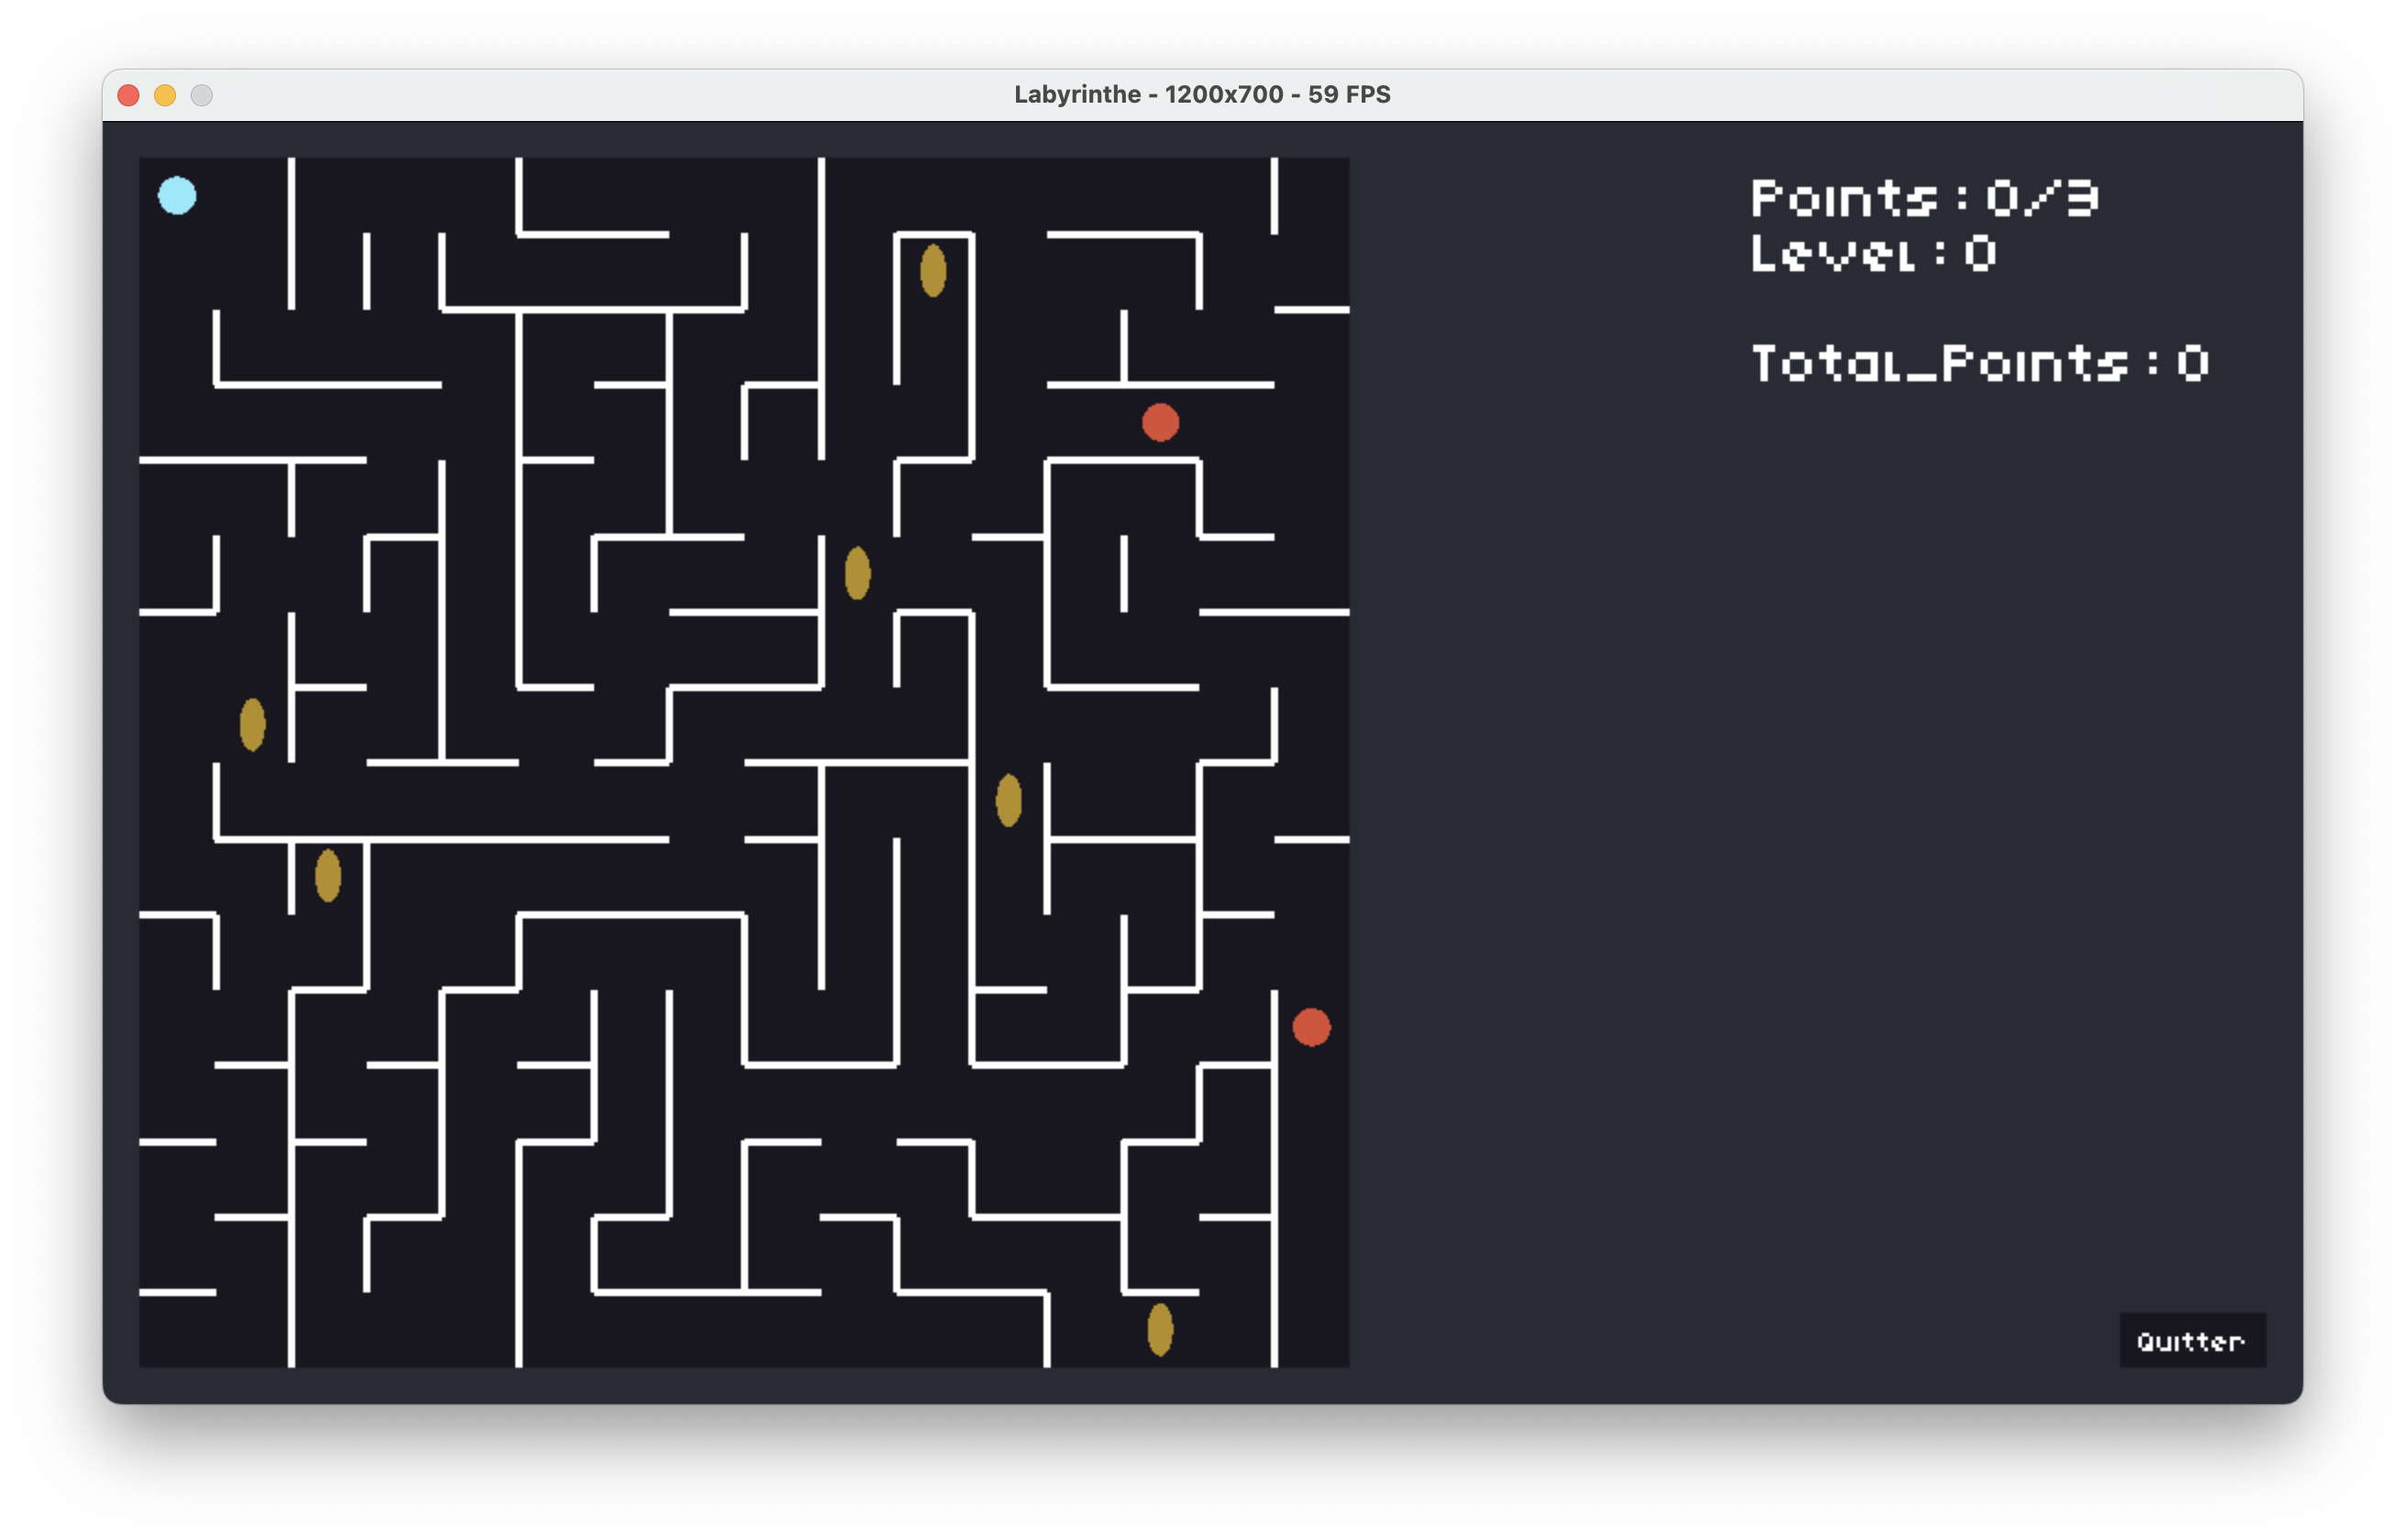
\includegraphics[width=\textwidth]{images/gamelevel0.png}
    \caption{Capture d'écran du premier niveau du jeu : le joueur doit ramasser trois points parmi les six disponibles tout en évitant deux ennemis}
\end{figure}

\begin{figure}[h]
    \centering
    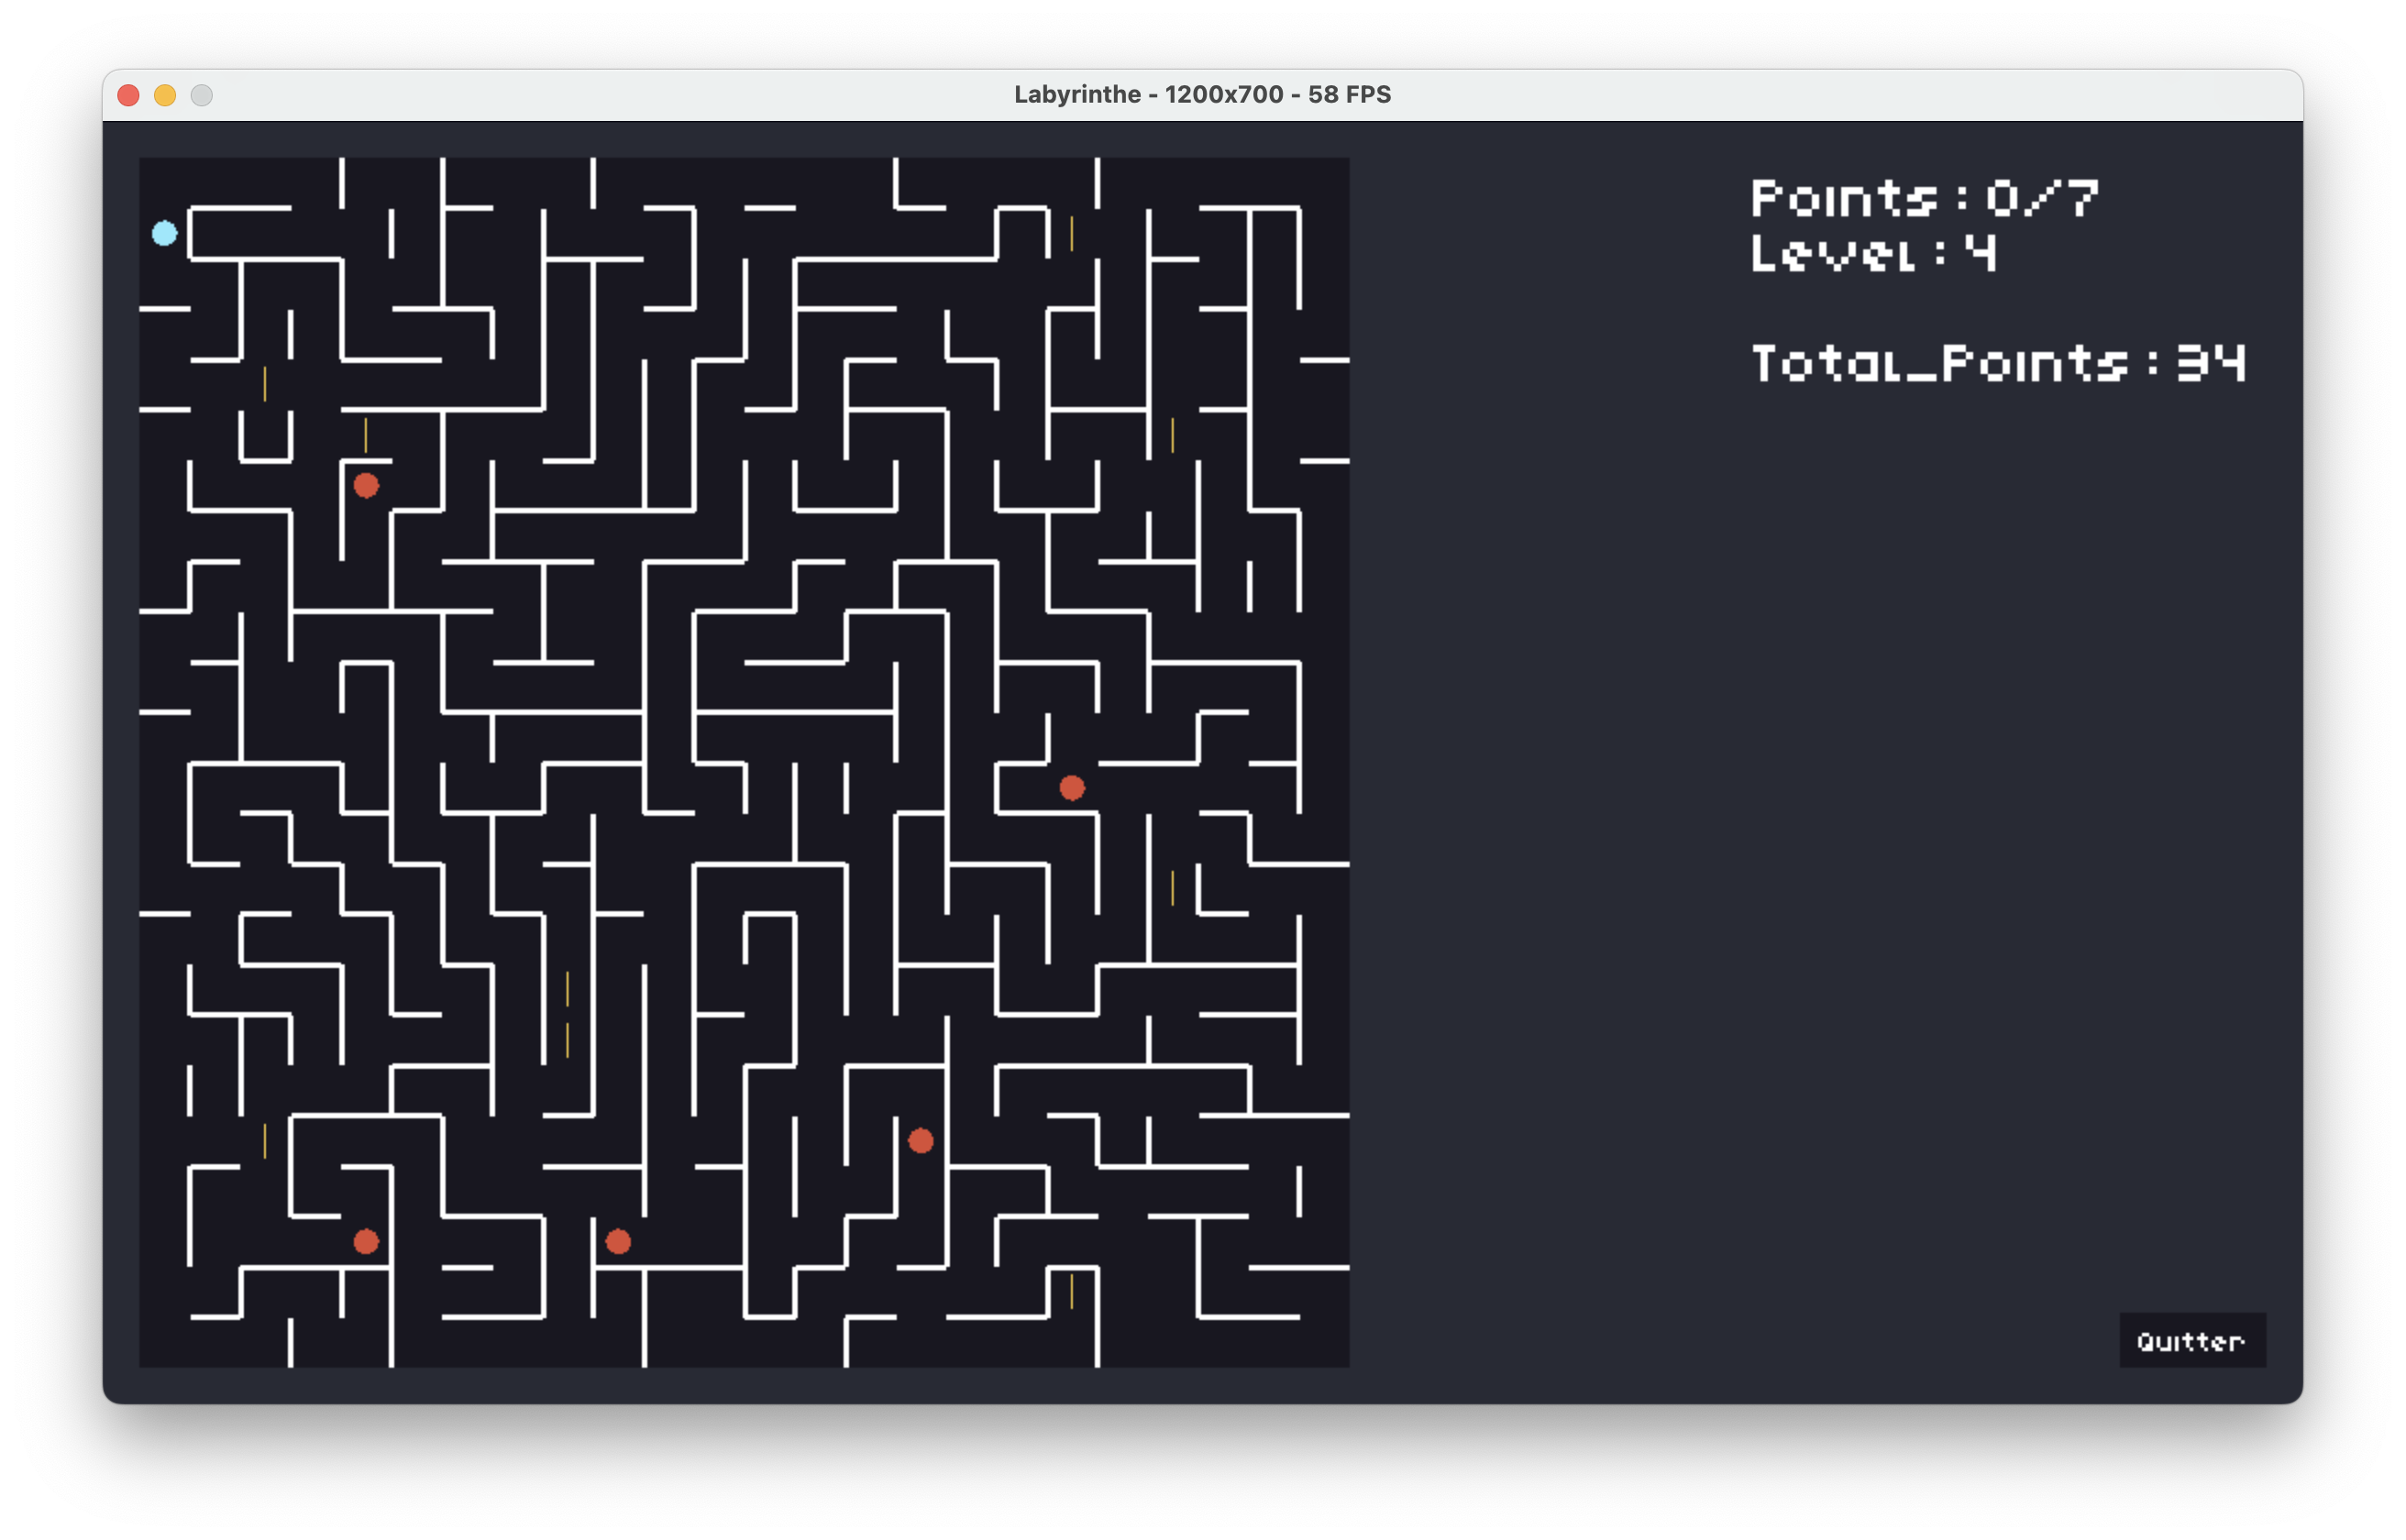
\includegraphics[width=\textwidth]{images/gamelevel4.png}
    \caption{Capture d'écran du cinquième niveau du jeu : le labyrinthe est plus grand, les ennemis et les points plus nombreux.}
\end{figure}

\begin{figure}[h]
    \centering
    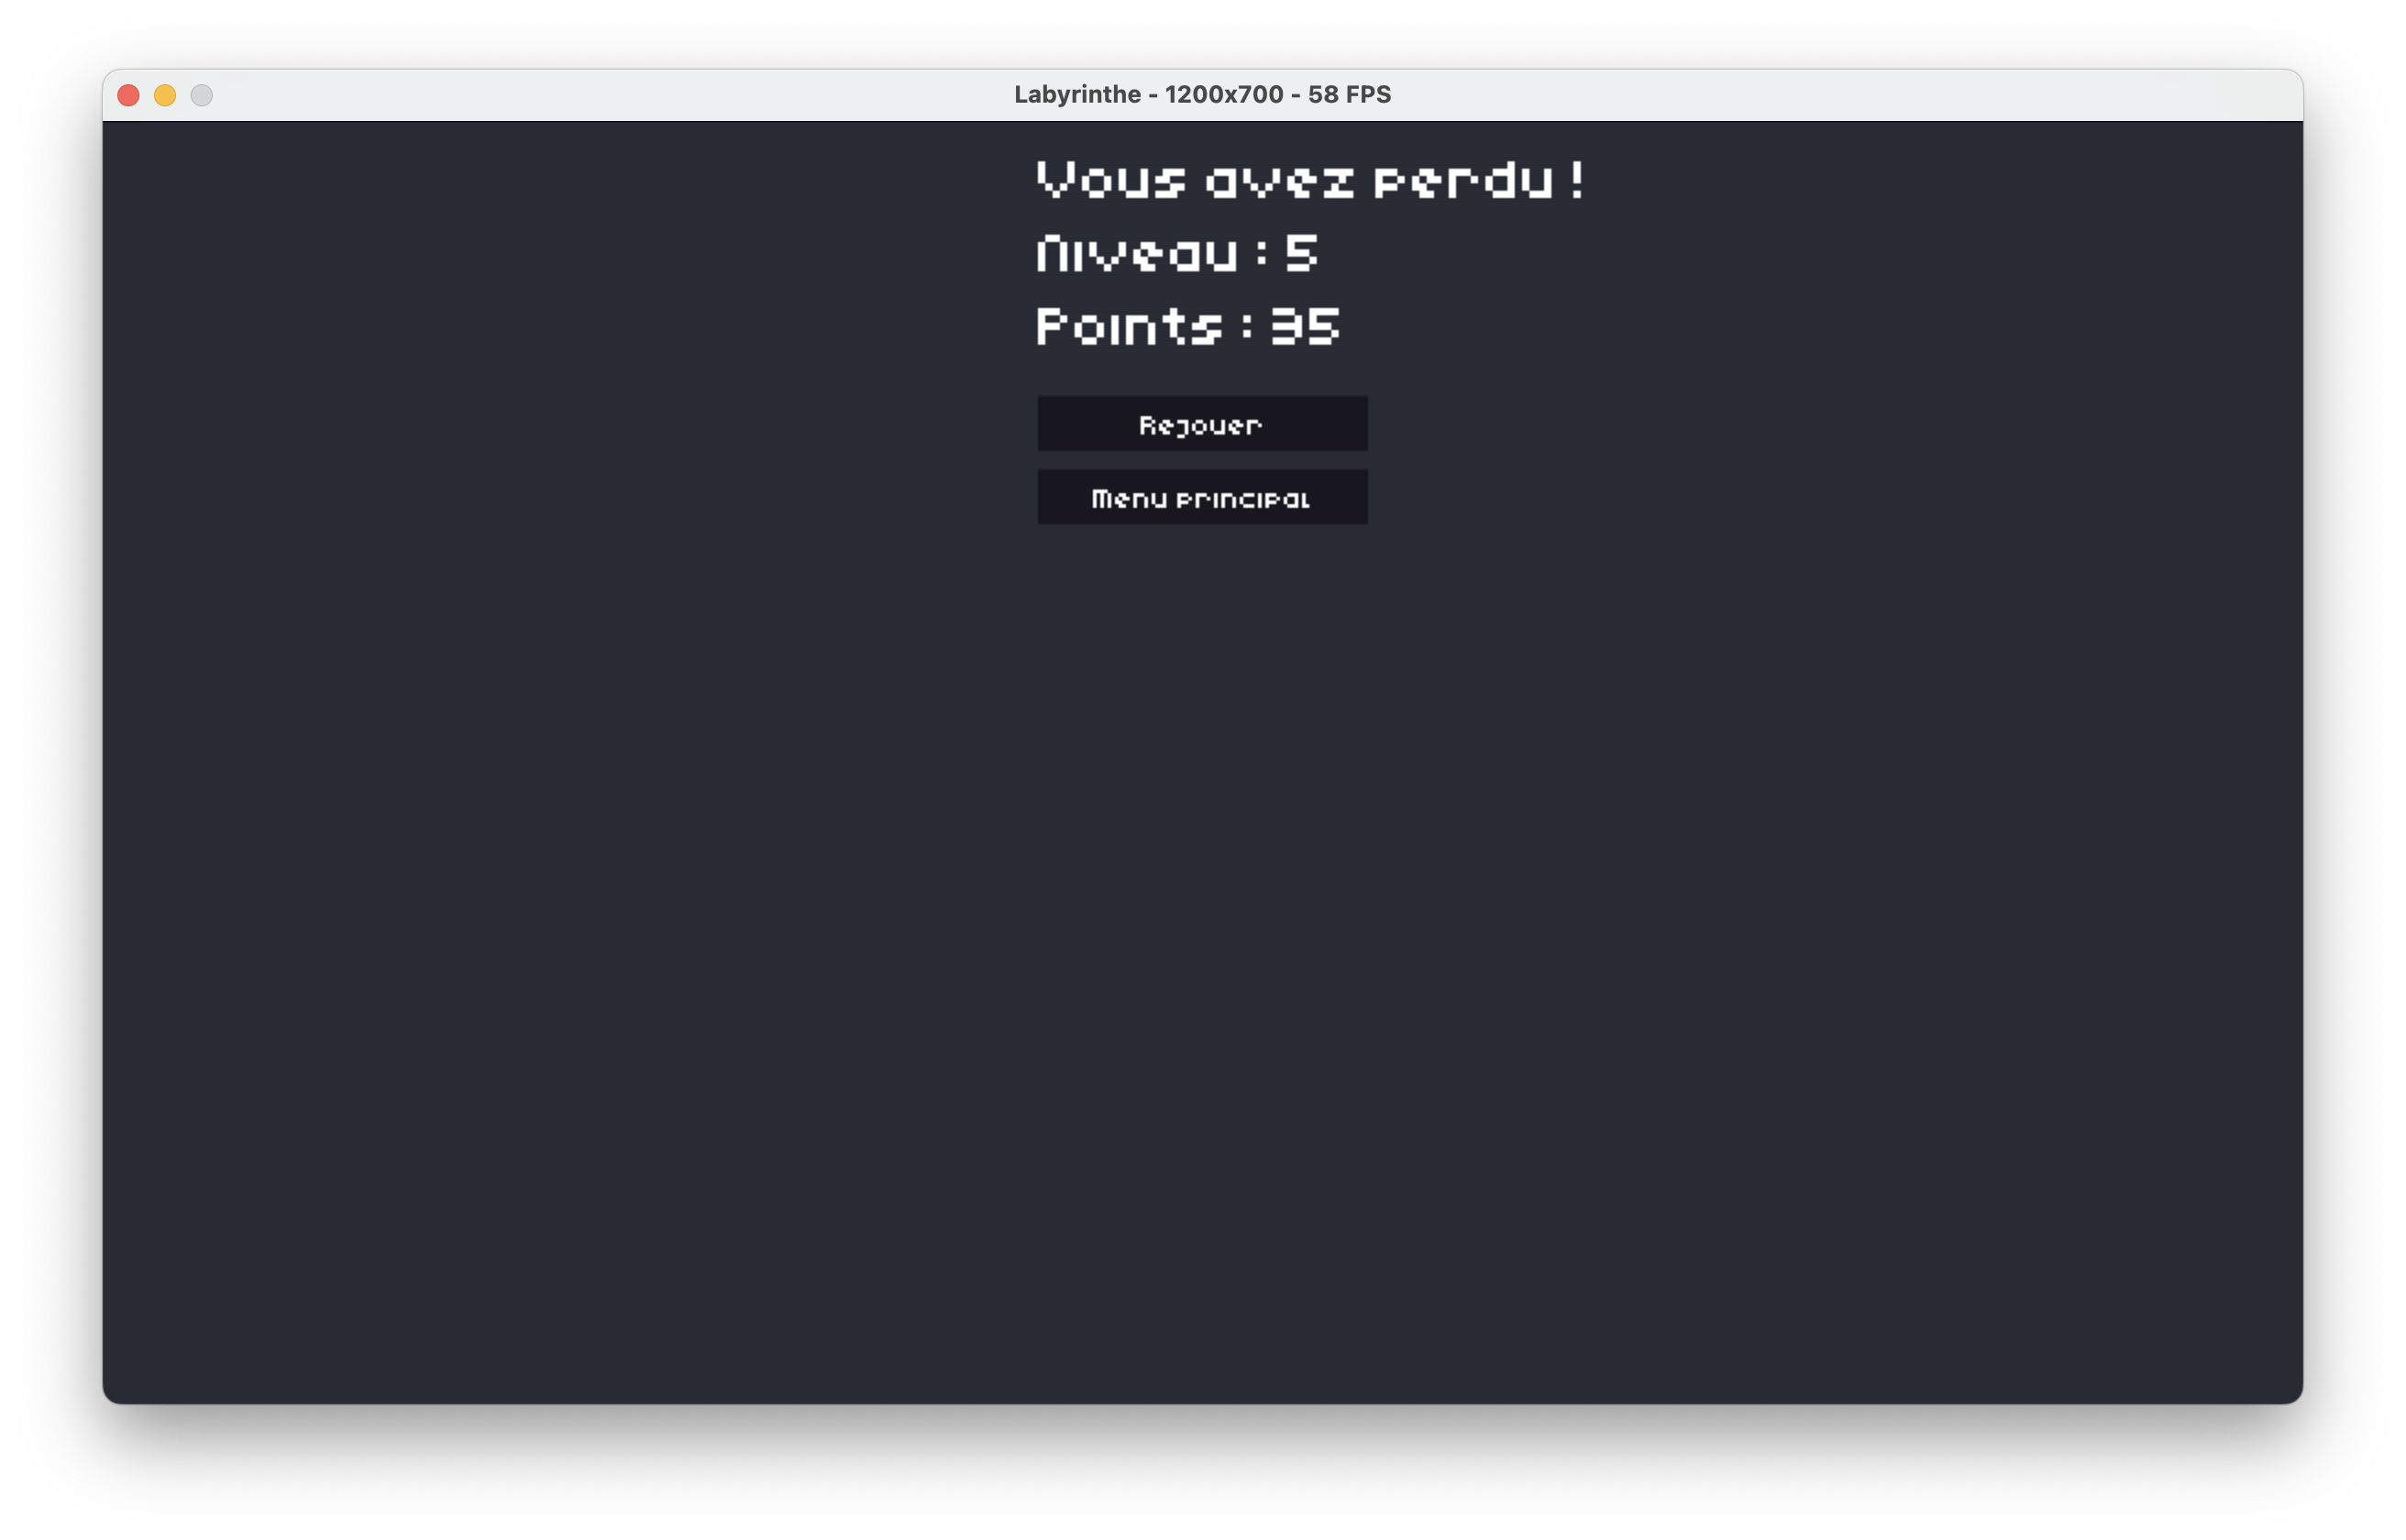
\includegraphics[width=\textwidth]{images/loosemenu.png}
    \caption{Capture d'écran du menu de fin de partie : le joueur peut consulter son score, recommencer ou retourner au menu principal.}
\end{figure}


Bien que très simple, le jeu est étonnamment amusant et équilibré : les ennemis suivent toujours un chemin quasi-optimal pour attraper le joueur, mais il est souvent possible de les éviter en anticipant leurs mouvements. Pour établir un score élevé, il est nécessaire d'avoir une vue d'ensemble du labyrinthe afin d'identifier les chemins les plus sûrs pour collecter les points et anticiper les ennemis. Il est par exemple dangereux de s'engager dans un long couloir ne présentant pas ou peu de boucles à proximité, car elles permettent de se sortir d'une situation où deux ennemis se rapprochent de part et d'autre.

\chapter{Implémentation}

Dans ce chapitre, nous allons décrire la structure du programme, ainsi que les différentes fonctionnalités que nous avons implémentées et les obstacles que nous avons rencontrés.

\section{Structure du programme}

Le programme que nous avons réalisé est divisé en plusieurs fichiers Python, chacun regroupant un certain nombre de fonctionnalités spécifiques.

Nous avons utilisé un paradigme de programmation orientée objet tout au long du projet, afin de créer des classes qui représentent les différents éléments du programme, comme les labyrinthes, les menus, les éléments graphiques, les entités évoluant au sein du jeu, etc.

Afin d'éviter de créer des conflits d'importation de type "importation circulaire" (deux fichiers s'importent mutuellement), la division du programme peut avoir lieu de façon assez naturelle, en isolant les classes utilisées à plusieurs endroits dans un fichier à part.

Cette façon de procéder encourage la réutilisation du code source, ce qui a beaucoup été fait dans ce projet, notamment pour les éléments graphiques et les labyrinthes en eux-même.

De nombreuses classes héritent de classes fournies par \texttt{pygame-ce}, ce qui permet de faciliter l'implémentation de certaines fonctionnalités, comme la gestion des événements, l'affichage des éléments graphiques, etc.

Ainsi, de façon générale, chaque classe qui représente un élément visible à l'écran est responsable de son propre affichage, de sa mise à jour, et de sa gestion des événements, le tout étant piloté par une classe principale \texttt{Menu} qui gère l'affichage des différents menus du programme.

Nous avons également fait le choix de stocker les constantes régulièrement utilisées dans un fichier à part, afin d'y avoir accès facilement et de pouvoir les modifier rapidement si besoin. Ce fichier peut également faire office de "configuration" du programme, en regroupant toutes les options modifiables par l'utilisateur.

\section{Classes, fonctions et méthodes principales}

\subsection{La classe \texttt{Labyrinthe}}

\subsubsection{Structure de donnée et méthodes utilitaires}

La classe \texttt{Labyrinthe} est la classe principale du programme, qui représente un labyrinthe. Elle contient toute la logique nécéssaire à la génération la résolution et l'affichage d'un labyrinthe à l'écran.

Elle hérite de la classe \texttt{pygame.sprite.Sprite}, ce qui lui fournit par défaut des attributs de taille, de position, une image, une forme, ainsi que des méthodes pour l'affichage et la mise à jour de l'objet.

Lors de l'initialisation, cette classe prend en paramètre la taille du labyrinthe, le facteur de bouclage, et les algorithmes de génération et de résolution à utiliser. Elle crée ensuite un labyrinthe vide et initialise les algorithmes.

Plutôt que de stocker les informations du labyrinthe sous forme de matrice ou de graphe, nous avons choisi de simplement stocker tous les murs qui le composent dans une liste, sous la forme d'un \texttt{tuple} des deux cases qu'il sépare.

Les cases sont quand à elles identifiées par un identifiant entier unique. Si on imagine le labyrinthe comme une grille, alors on peut numéroter chaque case de $0$ à $n^2 - 1$, où $n$ est la taille d'un côté du labyrinthe.

Ainsi, nous avons facilement pu implémenter de nombreuses méthodes utilitaires permettant d'ajouter ou de retirer des murs, d'obtenir une liste des cases adjacentes à une case donnée, de vérifier si un mur existe entre deux cases, etc. Ces méthodes sont utilisées par les algorithmes qui manipulent le labyrinthe.

\subsubsection{Génération et Résolution instantanées ou par étapes}

Lorsque nous avons commencé à travailler sur les algorithmes de génération et de résolution, nous avons instinctivement simplement créé des méthodes qui remplissaient leur rôle en une seule fois, c'est à dire des fonctions bloquantes qui ne permettaient pas d'observer le fonctionnement du programme au fur et à mesure.

Cette approche est efficace pour une première implémentation, mais notre objectif était de créer des visualisations interactives qui affichent toutes les données intéressantes afin de mieux comprendre le fonctionnement des algorithmes.

Ainsi, nous avons créé des méthodes alternatives en plus de celles qui existaient déjà, qui n'avancent l'algorithme sélectionné que d'une étape à la fois en tirant parti du fait que ces algorithmes sont basés sur des boucles. Ainsi, on peut afficher la nouvelle visualisation à chaque étape, en échange d'un temps d'exécution beaucoup plus long.

Cette façon de procéder a toutefois un inconvénient majeur : comme on génère ou résoud un labyrinthe avec plusieurs appels de fonctions, on ne peut plus utiliser de variables locales pour stocker des données essentielles comme la pile ou la liste de cases visitées présentes dans l'algorithme de \texttt{recursive backtracking}. Plus encore, les structures de données utilisées changent d'un algorithme à l'autre, tout comme les visualisations. Il était donc nécessaire de stocker ces données directement dans l'instance du Labyrinthe.

Nous aurions pu définir de nouvelles classes pour stocker ces données, mais comme leur utilisation est très spécifique, nous avons opté pour le choix de la simplicité et utilisé des dictionnaires. Lors de l'appel de la méthode de génération ou résolution, on choisit la bonne structure de donnée, le bon algorithme et la bonne visualisation à l'aide d'une simple structure \texttt{if-elif-else}. L'inconvénient principal de cette méthode est le fait qu'il est difficile d'ajouter de nouveaux algorithmes sans modifier d'autres morceaux de code sans réel lien fonctionnel, ce qui est considéré comme une mauvaise pratique.

\subsubsection{Interface et visualisation}

Les dernières méthodes intéressantes de la classe \texttt{Labyrinthe} sont celles qui permettent d'afficher le labyrinthe à l'écran.

En effet, le programme opère à une résolution fixée de 1200 par 700 pixels, et le labyrinthe à l'écran est censé occuper le même espace, quel que soit sa taille. Ainsi, l'approche logique aurait été de dessiner les éléments du labyrinthe en changeant la taille de chaque élément, mais nous avons décidé d'utiliser une astuce pour ne pas avoir à le faire.

Dans le fichier \texttt{constants.py}, nous avons défini une variable entière "Résolution du Labyrinthe" qui correspond à la taille d'une case du labyrinthe, en pixel. On peut constater que cette variable est fixe et est plutôt grande (120 pixels), ce qui peut sembler contre intuitif.

Au moment de générer l'image du labyrinthe, on le dessine sur une surface virtuelle en utilisant cette résolution, que l'on redimensionne ensuite pour l'afficher à l'écran. Ainsi, on obtient un labyrinthe de taille fixe, quelle que soit sa dimension, et on peut facilement le redimensionner pour l'afficher à l'écran où l'on veut, à la taille que l'on veut, sans nécessairement avoir à redimensionner chaque élément et surtout, sans avoir à le redessiner si il n'a pas changé.

En effet, afin d'optimiser les performances du programme, nous avons implémenter un système de "cache" qui permet de stocker l'image du labyrinthe au sein de l'instance, et de ne la redessiner que si le labyrinthe a changé depuis la dernière fois qu'il a été affiché (par exemple lorsque les algorithmes qui le modifient sont appelés).

On constate un gain de performances significatif en utilisant cette méthode, particulièrement dans des contextes où le labyrinthe ne change plus, comme lors de la résolution d'un labyrinthe déjà généré.

Afin de tirer parti au maximum de cette optimisation, la visualisation est donc dessinée sur une nouvelle surface virtuelle de la taille du labyrinthe. Cette surface est ensuite superposée à celle du labyrinthe, ce qui permet d'obtenir l'image finale.

Cette technique de "cache" est utilisé à plusieurs reprises dans le code, bien qu'elle ne soit réellement nécéssaire que dans ce contexte.

\subsection{Les classes \texttt{MenuFactory}, \texttt{Menu}, \texttt{Button} et \texttt{Text}}

Un grand nombre de classes du programme sont des menus, qui représentent chacun un écran spécifique (écran titre, écran de génération personnalisée, affichage du jeu, etc.). Afin de faciliter la création de ces menus, nous avons créé une classe \texttt{MenuFactory} qui permet de créer des menus sans répétition de code. Elle permet d'ajouter très facilement des éléments graphiques à un menu, de les positionner, de les afficher, de les mettre à jour, etc.


La classe \texttt{MenuFactory} est une classe abstraite qui définit les méthodes et les attributs communs à tous les menus du programme. Elle contient une méthode \texttt{update} qui met à jour les éléments graphiques du menu, une méthode \texttt{draw} qui affiche les éléments graphiques du menu à l'écran, et des méthodes \texttt{on\_click} et \texttt{on\_key} qui gèrent respectivement les clics de souris et les appuis de touches clavier.

Cette classe possède deux attributs, \texttt{elements} et \texttt{buttons}, qui sont des groupes de sprites contenant respectivement tous les éléments graphiques du menu, et tous les boutons du menu. Ces groupes de sprites sont utilisés pour afficher et mettre à jour les éléments graphiques du menu. Les groupes de sprites sont des classes fournies par \texttt{pygame-ce}, qui fonctionnent de façon assez similaire aux listes, mais qui permettent uniquement de stocker des objets de type \texttt{pygame.sprite.Sprite}. En contrepartie, il est possible d'appeler des méthodes sur l'ensemble des sprites stockés dans un groupe beaucoup plus rapidement qu'avec une liste.

Lorsque le menu est mis à jour, la méthode \texttt{update} est appelée, ce qui met à jour les éléments graphiques du menu. Cette méthode appelle ensuite la méthode \texttt{update} de chaque élément graphique du menu, ce qui permet de mettre à jour les éléments graphiques du menu. Enfin, la méthode \texttt{draw} est appelée, ce qui affiche les éléments graphiques du menu à l'écran.

Lorsqu'un clic de souris est détecté, la méthode \texttt{on\_click} est appelée, qui détermine si un bouton a été cliqué et si oui, lequel. Cette méthode tire profit du fait que les boutons sont stockés dans un groupe de sprites, ce qui permet de détecter très facilement des collisions avec un rectangle invisible placé à la position de la souris. Si un bouton est cliqué, la méthode \texttt{on\_click} du bouton est appelée, ce qui permet de définir le comportement du bouton.

Lorsqu'on veut ajouter un élément à un menu, on peut simplement l'instancier au sein de la méthode \texttt{\_\_init\_\_} de sa classe, puis l'ajouter au groupe correspondant. L'affichage et la mise à jour de l'élément seront alors gérés automatiquement par la classe \texttt{MenuFactory}.

Tous les écrans du programme sont des instances de classes qui héritent de la classe \texttt{MenuFactory}, et sont stockés dans une pile au sein de la classe \texttt{Menu}. Lorsqu'un clic de souris est détecté, la méthode \texttt{on\_click} de l'écran du dessus de la pile est appelée, ce qui permet de gérer les clics de souris de façon cohérente.

De la même façon, seul le menu en haut de la pile est mis à jour et dessiné à chaque frame, ce qui permet de garder en mémoire les écrans précédents sans les traiter inutilement.

\subsection{Les classes \texttt{Game}, \texttt{Character}, \texttt{Enemy} et \texttt{Point}}




\chapter*{Conclusion}
\addcontentsline{toc}{chapter}{Conclusion} % Add the chapter to the table of contents

Résumer les points clés du projet

Réiterer sur le but de ce projet et ce que la recherche dans ce domaine permet d'apporter à la science

Donner son impression générale par rapport à ce que nous a apporté le projet

\newpage % Start a new page for the bibliography
\renewcommand{\bibname}{Bibliographie} % Change the title of the bibliography section to "Références"

\bibliographystyle{unsrt} % Set the bibliography style. Change "plain" to the style you want to use.
\bibliography{references} % Include the bibliography file. Change "references" to the name of your .bib file.
\addcontentsline{toc}{chapter}{Bibliographie} % Add the chapter to the table of contents

\chapter*{Compte rendus hebdomadaires}
\addcontentsline{toc}{chapter}{Compte rendus hebdomadaires} % Add the chapter to the table of contents

\chapter*{Annexes}
\addcontentsline{toc}{chapter}{Annexes} % Add the chapter to the table of contents

\section*{Annexe 1 : Code source et installation}
\addcontentsline{toc}{section}{Annexe 1 : Code source et installation} % Add the section to the table of contents

\subsection*{Prérequis}

Afin de pouvoir installer et exécuter le programme, il est nécessaire de disposer des éléments suivants :
\begin{enumerate}
    \item Python 3.10 ou supérieur. Les versions antérieures n'ont pas été testées et ne sont pas garantie de fonctionner.
    \item Des notions de base avec l'interface en ligne de commande de votre système d'exploitation.
\end{enumerate}

\subsection*{Installation}

Afin d'obtenir le code source du programme et l'installer sur votre machine, veuillez suivre les instructions suivantes (également décrites dans le fichier \texttt{README.md} du dépôt Git) :

\begin{enumerate}
    \item Télécharger le code source du programme en suivant l'une des trois méthodes suivantes :
          \begin{itemize}
              \item Cloner le dépôt Git à l'aide de la commande suivante :
                    \begin{verbatim}
git clone https://github.com/HerbeMalveillante/ProjetPeiP24.git      
              \end{verbatim}
              \item Télécharger le code source sous forme d'archive ZIP en cliquant sur le bouton "Code" du dépôt Git, puis sur "Download ZIP".
              \item Obtenir le code source à partir du fichier ZIP fourni avec ce rapport.
          \end{itemize}
    \item Ouvrir un terminal et se placer dans le dossier contenant le code source du programme.
    \item Vérifier la version de Python utilisée dans le PATH à l'aide de la commande suivante :
          \begin{verbatim}
python3 --version
    \end{verbatim}
          Il est bon de noter que la commande permettant d'invoquer Python peut dépendre de votre système d'exploitation et/ou de votre installation de Python. Les commandes les plus courantes sont \texttt{python}, \texttt{python3} et \texttt{py}.
    \item (optionnel) Créer un environnement virtuel Python à l'aide de la commande suivante :
          \begin{verbatim}
python3 -m venv .envi

# activer l'environnement virtuel sur Unix
source .envi/bin/activate

# activer l'environnement virtuel sur Windows
.envi\Scripts\activate
    \end{verbatim}
    \item Installer les dépendances du programme à l'aide de la commande suivante :
          \begin{verbatim}
python3 -m pip install --upgrade pip
python3 -m pip install -r requirements.txt
    \end{verbatim}
          Veuillez noter que si une erreur liée à Pygame survient, il convient de vérifier que la version installée est bien la version "communauté" de Pygame (\texttt{pygame-ce}), et non la version officielle (\texttt{pygame}).

    \item Lancer le programme à l'aide de la commande suivante :
          \begin{verbatim}
python3 main.py
    \end{verbatim}

\end{enumerate}



\newpage

\begin{center}
    \Huge
    Projet Informatique : Labyrinthe
\end{center}

\section*{Résumé}

\blindtext

\section*{Mots-clés}

Labyrinthe, ajouter, d'autres, mots, clés

\section*{Abstract}
\blindtext

\section*{Keywords}

Labyrinth, add, other, keywords

\hrulefill

\vfill

\newcolumntype{Y}{>{\raggedleft\arraybackslash}X} % Redefine the X column type to align the text to the right

\begin{table}[h]
    \begin{tabularx}{\textwidth}{|X|Y|}
        \hline
        Encadrant académique              & Étudiants                               \\
        \textcolor{red}{Christophe Lenté} & \textcolor{red}{Pacôme Renimel--Lamiré} \\
                                          & \textcolor{red}{Esteban Laurent}        \\
        \hline
    \end{tabularx}
\end{table}



\end{document}